% ==============================================================================
% RapidBoxForest (RBF) — IEEE Transactions on Robotics submission source (EN).
% Standalone-compilable; generated tables/macros live under doc/paper/tro_rewrite_2026/generated/.
% ==============================================================================
\documentclass[journal]{IEEEtran}

% Load the silence package as early as possible to filter benign font and box
% warnings that are emitted during package/class loading in automated builds.
\RequirePackage{silence}
\WarningFilter{latexfont}{Font shape}
\WarningFilter{latexfont}{Some font shapes were not available}
\hbadness=10000
\vbadness=10000

% Font and micro-typography settings for XeLaTeX: prefer a Times-like
% text font that provides small-caps shapes and reliably defined bold shapes.
% These settings reduce missing-font-shape warnings and improve paragraph
% justification behaviour under XeLaTeX.
\usepackage{fontspec}
% Use the built-in Latin Modern family directly to avoid font discovery work
% during compilation on hosted services.
\setmainfont{Latin Modern Roman}[Ligatures=TeX,Scale=MatchLowercase]
\setsansfont{Latin Modern Sans}[Scale=MatchLowercase]
\setmonofont{Latin Modern Mono}[Scale=MatchLowercase]

% If the document uses \textsc extensively but the chosen font lacks OpenType
% small-caps, avoid generating TU/.../sc requests by mapping \textsc to an
% uppercase form instead of real small-caps shapes. Use a robust definition
\DeclareRobustCommand{\textsc}[1]{\textnormal{\MakeUppercase{#1}}}

% Loosen paragraph tolerance slightly to avoid underfull hbox warnings in
% narrow IEEE two-column layout while keeping good justification.
\tolerance=2000
\emergencystretch=2em
% Keep floats close to the text that introduces them.
\setcounter{topnumber}{4}
\setcounter{bottomnumber}{3}
\setcounter{totalnumber}{6}
\renewcommand{\topfraction}{0.92}
\renewcommand{\bottomfraction}{0.8}
\renewcommand{\textfraction}{0.05}
\renewcommand{\floatpagefraction}{0.85}
\renewcommand{\dbltopfraction}{0.9}
\renewcommand{\dblfloatpagefraction}{0.85}
\setlength{\textfloatsep}{5pt plus 1pt minus 2pt}
\setlength{\dbltextfloatsep}{6pt plus 1pt minus 2pt}
\setlength{\floatsep}{4pt plus 1pt minus 2pt}
\setlength{\intextsep}{5pt plus 1pt minus 2pt}
\setlength{\abovecaptionskip}{3pt}
\setlength{\belowcaptionskip}{0pt}
\setlength{\abovedisplayskip}{5pt plus 1pt minus 2pt}
\setlength{\belowdisplayskip}{5pt plus 1pt minus 2pt}
\setlength{\abovedisplayshortskip}{4pt plus 1pt minus 2pt}
\setlength{\belowdisplayshortskip}{4pt plus 1pt minus 2pt}
\setlength{\jot}{1pt}

\usepackage{amsmath,amssymb,amsfonts}
\usepackage{amsthm}
\usepackage{algorithm}
\usepackage{algorithmic}
\usepackage{afterpage}
\usepackage{booktabs}
\usepackage{dblfloatfix}
\usepackage{rotating}
\usepackage{graphicx}
\usepackage{capt-of}
\usepackage{placeins}
\usepackage{bm}
\usepackage{xr}
\usepackage{hyperref}
\usepackage{cleveref}
\usepackage{etoolbox}
\usepackage[inline]{enumitem}

\newtheorem{theorem}{Theorem}
\newtheorem{proposition}{Proposition}
\newtheorem{definition}{Definition}
\newtheorem{remark}{Remark}
\newtheorem{lemma}{Lemma}
\newtheorem{corollary}{Corollary}
\newtheorem{assumption}{Assumption}

\input{generated/macros.tex}
\IfFileExists{generated/macros_sbf.tex}{\input{generated/macros_sbf.tex}}{}
\IfFileExists{generated/tro_macros.tex}{% Auto-generated by experiments/tro2026_generate_tables.py
\newcommand{\TroAuditedGcsAuditPass}{--/--}
\newcommand{\TroExpandedGcsAuditPass}{--/--}
\newcommand{\TroDirectGcsAuditPass}{--/--}
\newcommand{\TroSbfBuildMean}{--}
\newcommand{\TroSbfBoxMean}{--}
\newcommand{\TroPaperAuditPass}{--/--}
\newcommand{\TroRbfOnlyEFiveLeafFk}{--}
\newcommand{\TroRbfOnlyEFiveEvidence}{--}
\newcommand{\TroRbfOnlyEFiveFirstWall}{--}
\newcommand{\TroRbfOnlyEFiveReopenWall}{--}
\newcommand{\TroRbfOnlyEFiveReopenReuse}{--}
\newcommand{\TroRbfOnlySweepBestEnvelope}{--}
\newcommand{\TroRbfOnlySweepBestBudget}{--}
\newcommand{\TroRbfOnlySweepBestBuild}{--}
\newcommand{\TroRbfOnlySweepBestQueryMs}{--}
\newcommand{\TroRbfOnlySweepBestReuse}{--}
\newcommand{\TroRbfOnlySweepFullPassRows}{--}
\newcommand{\TroRbfOnlyShelfWarmBuild}{--}
\newcommand{\TroRbfOnlyShelfWarmQueryMs}{--}
\newcommand{\TroRbfOnlyShelfWarmExternalReuse}{--}
\newcommand{\TroRbfOnlyEFourWarmBuildMin}{--}
\newcommand{\TroRbfOnlyEFourWarmBuildMax}{--}
\newcommand{\TroRbfOnlyEFourWarmQueryMinMs}{--}
\newcommand{\TroRbfOnlyEFourWarmQueryMaxMs}{--}
\newcommand{\TroRbfOnlyEFourWarmAuditMin}{--}
\renewcommand{\TroAuditedGcsAuditPass}{3/5}
\renewcommand{\TroExpandedGcsAuditPass}{0/4}
\renewcommand{\TroDirectGcsAuditPass}{0/5}
\renewcommand{\TroSbfBuildMean}{0.9393}
\renewcommand{\TroSbfBoxMean}{150.90}
\renewcommand{\TroPaperAuditPass}{663/668}
\renewcommand{\TroRbfOnlyEFiveLeafFk}{262144}
\renewcommand{\TroRbfOnlyEFiveEvidence}{524287}
\renewcommand{\TroRbfOnlyEFiveFirstWall}{20.17}
\renewcommand{\TroRbfOnlyEFiveReopenWall}{1.505}
\renewcommand{\TroRbfOnlyEFiveReopenReuse}{262144}
\renewcommand{\TroRbfOnlySweepBestEnvelope}{LinkIAABB}
\renewcommand{\TroRbfOnlySweepBestBudget}{256}
\renewcommand{\TroRbfOnlySweepBestBuild}{0.0032}
\renewcommand{\TroRbfOnlySweepBestQueryMs}{46.05}
\renewcommand{\TroRbfOnlySweepBestReuse}{205.00}
\renewcommand{\TroRbfOnlySweepFullPassRows}{6}
\renewcommand{\TroRbfOnlyShelfWarmBuild}{1.588}
\renewcommand{\TroRbfOnlyShelfWarmQueryMs}{3.568}
\renewcommand{\TroRbfOnlyShelfWarmExternalReuse}{7201}
\renewcommand{\TroRbfOnlyEFourWarmBuildMin}{0.0016}
\renewcommand{\TroRbfOnlyEFourWarmBuildMax}{0.5569}
\renewcommand{\TroRbfOnlyEFourWarmQueryMinMs}{0.6615}
\renewcommand{\TroRbfOnlyEFourWarmQueryMaxMs}{3.536}
\renewcommand{\TroRbfOnlyEFourWarmAuditMin}{100.00}
}{}

\newcommand{\rbf}{\textsc{RBF}}
\newcommand{\iAABB}{\ensuremath{\mathrm{iAABB}}}
\newcommand{\Real}{\ensuremath{\mathbb{R}}}
\newcommand{\Cfree}{\ensuremath{\mathcal{C}_{\mathrm{free}}}}
\newcommand{\calO}{\ensuremath{\mathcal{O}}}
\newcommand{\Q}{\ensuremath{\mathcal{Q}}}
\newcommand{\etal}{\textit{et al.}}
\renewcommand{\algorithmicrequire}{\textbf{Input:}}
\renewcommand{\algorithmicensure}{\textbf{Output:}}
\newcommand{\algcommentline}[1]{\STATE \textit{#1}}
\newcommand{\procname}[1]{\operatorname{#1}}

\newcommand{\TableFontStepUp}{%
  \let\TableOrigTiny\tiny
  \let\TableOrigScriptSize\scriptsize
  \let\TableOrigFootnoteSize\footnotesize
  \let\TableOrigSmall\small
  \renewcommand{\tiny}{\TableOrigScriptSize}
  \renewcommand{\scriptsize}{\TableOrigFootnoteSize}
  \renewcommand{\footnotesize}{\TableOrigSmall}
  \renewcommand{\small}{\normalsize}
}
\AtBeginEnvironment{table}{\TableFontStepUp}
\AtBeginEnvironment{table*}{\TableFontStepUp}
\AtBeginEnvironment{sidewaystable}{\TableFontStepUp}

\begin{document}

\title{RapidBoxForest:\\ Link-Envelope-Guided Box Forests for Fast Multi-Query Manipulation}

\author{TIAN,~Yu and Ren,~Hongliang%
\thanks{The authors are with the Department of Electronic Engineering,
The Chinese University of Hong Kong (CUHK), Hong Kong SAR, China.
E-mail: \texttt{ty1997@link.cuhk.edu.hk}.}}

\maketitle

\begin{abstract}
Fast repeated-query manipulation benefits from reusable volumetric planning
structure, but high-quality IRIS-style convex regions are expensive to construct
and rebuild. This paper presents RapidBoxForest (\rbf{}), a link-envelope-guided
box-forest planner for fast multi-query manipulation. The central geometric primitive maps endpoint interval envelopes to link
interval envelopes via capsule Minkowski decomposition and convex-hull generator
bounding applied to \emph{$C$-space box validation and multi-query reuse}:
endpoint interval envelopes bound rounded-link endpoint motion over a joint box,
and a radius-lifted link envelope provides an inexpensive filter for box
validation and collision rejection. A rapidly-exploring random tree
(RRT)-inspired grower builds a scene-specific box forest into a queryable
corridor graph, and a Lifelong Envelope Cache Tree (LECT) selectively caches
kinematics-keyed envelope records when replay is cheaper than recomputation. On the canonical Shelf+IIWA workload and on balanced IIWA,
UR5, and Panda easy/medium/hard random scenes, RBF-SH achieves reusable build
times of 0.15--1.1~s and online query times below 0.11~s, with final-audited
path lengths competitive with sampling-based baselines at a fraction of the
reusable build cost. Secondary mechanism studies quantify endpoint-source and
link-envelope representation trade-offs and show that LECT prewarm provides
measurable cross-scene gains. The results position link-envelope-guided box
forests as a practical multi-query planning system with an optional conservative
corridor validation mode. The accompanying artifact provides the full
implementation and reproduction instructions.
\end{abstract}

\begin{IEEEkeywords}
Motion planning, multi-query planning, link interval envelopes, box-region planning, final audit.
\end{IEEEkeywords}

% ==============================================================================
\section{Introduction}\label{sec:intro}

Motion planning for high-degree-of-freedom (DOF) manipulators becomes
especially demanding when a system must answer many related queries rather than
one isolated instance. In warehouses, packing cells, and shared workcells,
robot kinematics stay fixed while obstacles, task endpoints, or local scene
edits change. The central question is how to construct reusable $C$-space
planning structure quickly enough that repeated queries can benefit from
region-level search without paying a large scene-specific preprocessing cost.

Iterative Regional Inflation by Semidefinite Programming (IRIS) and
Graph-of-Convex-Sets (GCS) methods show why free-region construction is
valuable: once good convex regions are available, graph search or convex
optimization can produce high-quality motions over those regions
\cite{deits2015computing,marcucci2023motion,marcucci2024shortest}. The
limitation is construction cost. In high-dimensional manipulator scenes,
inflating and validating high-quality convex regions can dominate the planning
budget and must often be repeated when the scene changes. Sampling-based planners such as probabilistic roadmap (PRM) and
rapidly-exploring random tree (RRT) methods avoid this region-construction cost
\cite{lavalle2006planning,lavalle1998rapidly,kavraki1996probabilistic,
karaman2011sampling}, but their reusable structures are usually zero-volume
graphs, so repeated queries still pay for local collision checking and do not
obtain a reusable free-region cover.

\rbf{} targets a different design point by constructing simpler box regions
quickly.
Instead of inflating general polytopes, it grows axis-aligned boxes in
configuration space, connects accepted boxes into a graph, and answers later
queries by searching the resulting box corridor. This trades per-region
expressivity and sometimes path length for cheap construction, simple
adjacency, and direct reuse across many queries. The intended claim is a
system-level one: a fast box-region planning pipeline can be a useful
final-audited alternative when multi-query latency matters more than obtaining
the shortest path from a more expensive region decomposition.

The key technical ingredient is a link interval envelope computed from endpoint
interval envelopes. For rounded link models, \rbf{} reduces link motion over a
joint box to the motion of a zero-radius centerline plus a final radius lift.
Endpoint interval envelopes bound the endpoint trajectories over the joint box;
link interval envelopes then enclose the swept rounded link and can be stored as
axis-aligned bounding boxes (AABBs), $k$-DOP slabs, or SupportHull records. Strict interval sources provide an
optional conservative validation path, while tighter practical sources are used
as fast filters and discharged by the same final scene audit used for all
reported planners.

On top of this geometric primitive, the grower borrows the rapid
frontier-expansion idea of RRT: samples choose useful frontiers, a local region
oracle materializes a free box around the projected seed, and accepted boxes
extend a connected box forest. The result is also an adaptive cell-decomposition
view of manipulator $C$-space, but one biased toward the regions needed by the
current repeated-query workload. A Lifelong Envelope Cache Tree (LECT) then memoizes scene-independent endpoint
and link-envelope evidence keyed by robot kinematics and joint intervals; it is
an acceleration layer for repeated materialization, not a separate planning
claim.

The evaluation therefore asks where this envelope-based box forest lies on the
final-audited time/path-quality frontier of the implemented pipelines. The main
axes are reusable build time, online query time, fixed-resolution audited
success, path length, amortization, and scene/robot variation. The conservative
box-corridor statement is kept separate from the main comparisons because it
requires both strict validation and path containment in the validated box union,
whereas the reported paths may be changed by the common post-processing step.
Endpoint/link
envelope studies and LECT replay are reported to explain construction cost, with
LECT treated as an optimization layer. IRIS-NP+GCS is used as an important
pipeline baseline under the same workload-level seeds used by the other
planners: manually selected reference anchors in the Shelf+IIWA scene and fixed
random seeds in the random-scene study.

We therefore position the paper as a planning-systems contribution enabled by a
geometry primitive. The endpoint-to-link envelope is the main geometric idea;
the planner and artifact show how that primitive supports a reproducible
low-build-cost multi-query design point under final audit.

\textbf{The paper's main contribution is a reproducible final-audited
multi-query planning system and its measured design point. It is supported by
three concrete elements:}
\begin{enumerate}[nosep]
  \item \emph{An endpoint-to-link envelope primitive for $C$-space box validation.}
  Capsule Minkowski decomposition and convex-hull generator bounding are
  individually classical facts already combined in articulated-body CCD
  work~\cite{redon2004ccd_avatar,redon2005fast_artic,zhang2007taylor}.
  \rbf{} applies this two-step pipeline to \emph{$C$-space box growth and
  multi-query reuse}: a switchable endpoint source family---AA-backed
  interval forward kinematics (IFK), hierarchical IFK (HIFK),
  CritSample, analytical extrema---compact
  per-representation link records (AABB, KDOP26, SupportHull) for staged
  filtering, and a kinematic-keyed LECT cache for cross-scene envelope reuse.
  No prior work has been found applying this pipeline to $C$-space box
  validation or multi-query planning reuse
  (\cref{sec:link_envelopes,tab:tro_main_evidence_validation,tab:tro_link_envelope_widthwise}).

  \item \emph{A self-contained link-envelope-guided box-forest planner.}
  Scene-specific $C$-space box forests are grown through seeded frontier
  expansion, consolidated into a connected corridor graph, and queried by
  graph search and local refinement. LECT provides an optional
  kinematic-keyed cache for repeated envelope materialization across builds
  (\cref{sec:lect,sec:forest,tab:tro_main_lect_reuse}).

  \item \emph{A scoped final-audited design-point evaluation.}
  Shelf+IIWA and balanced IIWA/UR5/Panda scenes are evaluated under common
  post-processing and fixed-resolution final audit. \rbf{} achieves low
  reusable build/query cost with near-baseline audited path lengths; path
  quality improvements over the strongest baselines and grower-strategy
  ablations remain future work
  (\cref{fig:tro_shelf_anytime_tradeoff,fig:tro_random_anytime_tradeoff,tab:tro_main_shelf_best_tradeoff,tab:tro_main_random_best_tradeoff}).
\end{enumerate}

The paper's evidence chain is: \Cref{sec:link_envelopes} develops the endpoint
and link interval-envelope primitive for fast box validation; \cref{sec:lect}
describes the cache optimization that reuses expensive envelope records;
\cref{sec:forest} turns link-envelope-filtered boxes into a rapidly expanding
box-forest planner; and \cref{sec:exp} evaluates the resulting final-audited
build/query and path-quality trade-offs as implemented pipeline design points
with IRIS-NP+GCS, PRM, RRTConnect, and BIT* as contextual baselines.

\begin{figure*}[t]
  \centering
  
\includegraphics[width=0.97\textwidth]{figures/framework.png}
  \caption{\rbf{} pipeline for link-envelope-guided multi-query planning. Top: endpoint interval envelopes induce link interval envelopes over a $C$-space box. Middle: LECT optionally reuses kinematics-keyed endpoint and link-envelope records across repeated builds. Bottom: scene filtering and an RRT-inspired grower expand a connected box-region forest for lightweight corridor queries and final audit.}
  \label{fig:linkiaabb}
\end{figure*}
% ==============================================================================
\section{Related Work}\label{sec:related}

\subsection{Convex Region Planning and Graphs of Convex Sets}

Convex region planners approach motion planning by constructing a certified cover
of free space and then solving graph search or convex optimization on top of
that cover. IRIS introduced the now-standard idea of computing large
collision-free convex regions by alternating separating hyperplanes and region
inflation~\cite{deits2015computing}. Later work extended the same line into
configuration space, improved region quality, or improved graph compactness
through visibility-graph and clique-cover constructions~\cite{amice2022finding,
petersen2023growing,werner2024approximating}. Marcucci \etal{} made the
Graph-of-Convex-Sets formulation particularly influential by showing that motion
planning can be cast as optimization over a graph of certified convex
regions~\cite{marcucci2023motion,marcucci2024shortest}.

\rbf{} is aligned with this family in objective but not in geometric primitive:
it uses axis-aligned boxes in $C$-space rather than general polytopes, trading
per-region expressivity for lower build overhead and simpler adjacency
bookkeeping. The resulting cover is coarser than a high-quality convex
decomposition, but it avoids repeated hyperplane-based region inflation and is
easier to rebuild under repeated-query workloads. The comparison in this paper
therefore concerns fast reusable free-region construction versus tighter, more
scene-coupled regional convexification, rather than box and polytope
representations in isolation.

\subsection{Swept Volume Approximation and Capsule Geometry}

Computing the swept volume of a moving rigid body has been studied extensively
in computational geometry and computer-aided manufacturing (CAM)
communities~\cite{blackmore1992swept,abdel2006swept}.
For a convex body $P = \operatorname{conv}(v_1,\dots,v_m)$, bounding each
generator trajectory by a conservative outer set $\widehat{\Gamma}_i(I)$ yields
\[
  \mathcal{S}_I(P) \subseteq \operatorname{conv}\!\Bigl(\bigcup_i \widehat{\Gamma}_i(I)\Bigr),
\]
a bound that is implicit in oriented bounding box (OBB) tree construction for
swept mesh primitives~\cite{gottschalk1996obbtree}.

For capsule links this bound reduces to bounding only the two segment endpoints.
The Proximity Query Package (PQP) exploits exactly this Minkowski decomposition
($C = S \oplus B_2(r)$, sweep of $C$ reduces to sweep of $S$ plus radius
lift)~\cite{larsen1999fast}; GJK and its robust implementation by van den
Bergen apply the same identity for distance queries~\cite{gilbert1988fast,
bergen1999gjk}; the Flexible Collision Library (FCL) generalises the swept-sphere interface to
a full collision library~\cite{pan2012fcl}.

\subsection{Interval Forward Kinematics and the CCD Endpoint-Bounding Pipeline}

Interval arithmetic~\cite{moore2009introduction,jaulin2001applied} provides
inclusion-monotone enclosures of real-valued functions over parameter intervals.
Snyder applied interval arithmetic to parametric geometry to compute
conservative bounding boxes for curves and surfaces without mesh
sampling~\cite{snyder1992interval}. Merlet extended DH-chain interval
propagation to certified workspace analysis for parallel and serial
manipulators~\cite{merlet2004solving,merlet2009interval}.

These ideas meet directly in the continuous collision detection (CCD) literature
for articulated bodies. Redon, Kim, Lin, and Manocha~\cite{redon2004ccd_avatar}
model each robot limb as a line-swept sphere (LSS, i.e.~capsule) and
propagate interval Denavit-Hartenberg (DH) transforms along the kinematic
chain to obtain \emph{interval vectors bounding the two LSS endpoint positions}
over the
motion time step; the swept capsule is then bounded by padding the endpoint
bounding box with the link radius. This is explicitly the two-step pipeline
%
\begin{center}
  \emph{interval FK endpoint bounding}
  $\;\longrightarrow\;$
  $\operatorname{bbox}([\mathbf{p}_i]\cup[\mathbf{p}_{i+1}]) \oplus B_2(r)$
  $=$ \emph{link swept-capsule bound}
\end{center}
%
that is the geometric core of \rbf{}.
The journal extension by Redon, Lin, Manocha, and Kim~\cite{redon2005fast_artic}
applies the same framework to general robot arms and kinematic trees; that work
has accumulated over 240 citations and is a standard CCD reference.
Zhang \etal{}~\cite{zhang2007taylor} replace interval arithmetic with Taylor
models in the same pipeline to reduce wrapping errors, analogous to how
\rbf{}'s CritSample and analytical sources tighten the IFK bound.
Schwarzer \etal{}~\cite{schwarzer2005adaptive} address a multi-query motivation
similar to \rbf{}'s---reusing collision evidence across planning calls---but at
the path-segment level rather than as volumetric $C$-space records.
Corrales \etal{}~\cite{corrales2011ssl} apply sphere-swept line (SSL) bounding
volumes dynamically for human--robot safety monitoring using the same
structural observation that
bounding a capsule's motion reduces to bounding its two endpoints.

\subsection{Novelty Boundary: Prior CCD vs.\ \rbf{}}
\label{sec:related_novelty}

The two-step endpoint-interval-to-swept-capsule pipeline is therefore
unambiguously present in the CCD literature for time-step motion.
The differences that motivate the \rbf{} contribution claim are:
\begin{enumerate*}[label=(\alph*)]
  \item the parameter domain is a \emph{$C$-space joint-box interval} rather
    than a trajectory time step, so the goal is to classify whether \emph{any}
    configuration in the box is collision-free, not whether a single given path
    collides;
  \item the endpoint source is a switchable interface---IFK (conservative),
    CritSample (practical), and analytical extrema (tightest)---rather than a
    fixed algorithm, allowing the conservative vs.\ performance trade-off to be
    controlled without changing the link-representation or planner layers;
  \item compact per-representation link records (AABB, KDOP26, SupportHull) are
    organised for staged filtering during box growth, a knob absent from CCD
    libraries; and
  \item the endpoint and link envelope records are organised in LECT, a
    persistent \emph{kinematic-keyed} cache that reuses evidence across
    multi-query builds in related scenes, a reuse level not addressed by CCD
    libraries or path-segment caches.
\end{enumerate*}
No prior work has been found that applies the two-step endpoint bounding
pipeline to $C$-space box growth or to multi-query volumetric planning reuse.
\rbf{} is complementary to the CCD stack: link envelopes reduce repeated
geometric work on candidate boxes, while discrete scene checks remain the final
authority for the reported paths.

\subsection{Multi-Query Reuse and Adaptive Configuration-Space Decomposition}

Multi-query planners typically amortize effort by reusing a graph structure such
as a roadmap. PRM is the classical example: build a connectivity graph once and
reuse it for many start-goal pairs~\cite{kavraki1996probabilistic,
bohlin2000path}. LazyPRM, lazy edge checking, and certificate-based planners
postpone or cache edge validation so that online search does not repeatedly
evaluate the same discrete local connections~\cite{dellin2016unifying,
schmerling2015optimal}. Experience-based and trajectory-library systems reuse
prior solutions or local motion snippets, often as initialization or bias for a
new query rather than as a conservative decomposition of a region of
configuration space~\cite{coleman2014moveit}.

\rbf{} operates at a different reuse level. It grows and reuses volumetric boxes
rather than only paths, binary collision outcomes, or zero-volume edges.
PRM-like methods reuse connectivity and must revalidate affected edges after
scene changes. Convex-region planners reuse higher-quality regions, but those
regions are usually coupled to the obstacle layout in which they were
constructed.

The method also inherits the central idea of adaptive cell decomposition and
subdivision planning: represent free space by cells, split cells where the
current evidence is insufficient, and search the adjacency graph induced by the
accepted cells~\cite{lozanoperez1983spatial,brooks1985subdivision}. The
difference is the operating regime. Classical cell-decomposition examples are
often low-dimensional workspace or explicit $C$-space constructions, whereas
\rbf{} applies the same adaptive-cell idea to high-dimensional manipulator
$C$-space through a link-envelope oracle. Scene-specific obstacle filtering
is layered on top of reusable kinematic envelope evidence, with LECT available
only as a cache for expensive records. The trade-off is explicit: \rbf{} accepts
axis-aligned boxes and over-approximation in exchange for simple validation,
adjacency maintenance, and repeated-query throughput.

\subsection{Sampling-Based Planning and Trajectory Optimization}

Sampling-based planners remain standard baselines when the goal is to solve
a single query quickly. RRTConnect is particularly effective in manipulator
planning because bidirectional growth often succeeds with very little global
structure~\cite{kuffner2000rrt}. Asymptotically optimal and
informed variants such as RRT*, Batch Informed Trees (BIT*), and Fast Marching
Tree (FMT*) improve path quality and search efficiency when more time is
available~\cite{karaman2011sampling,
gammell2015batch,gammell2018informed,janson2015fmt}. The Open Motion Planning
Library (OMPL) has made these methods easy to deploy and benchmark in a common
software stack~\cite{sucan2012ompl,
moll2015benchmarking}. However, standard RRT variants produce single-use
zero-volume evidence and typically restart from scratch on the next query.

By contrast, \rbf{} uses rapidly exploring, adaptive expansion to sample and
materialize $C$-space boxes from the envelope oracle, producing a volumetric
corridor structure that can be queried repeatedly within the same environment.
Trajectory optimizers address a different stage of the pipeline. CHOMP, STOMP,
TrajOpt, and Gaussian-process motion planners refine an initial path by local
descent or sequential convex optimization~\cite{ratliff2009chomp,
kalakrishnan2011stomp,schulman2014motion,mukadam2018gpmp2}. \rbf{} uses these
methods as complementary points of comparison: its aim is to provide a
reusable volumetric backbone on which graph search and local post-processing
can operate.

% ==============================================================================
\section{Link Interval Envelopes}\label{sec:link_envelopes}

This section develops the main geometric primitive used by \rbf{}: a map from a
manipulator joint box to compact link interval envelopes. The goal is to make
box validation cheap enough for repeated-query planning. A strict interval
source gives a conservative validation option, while tighter sampled or
support-based variants are practical filters whose reported paths are discharged
by the common final audit. Thus the strongest free-region statement in this
section is conditional on the conservative source and on paths remaining inside
the validated box union; the main planning experiments report final-audited
performance separately. The construction first bounds endpoint trajectories and
then applies a constant-radius lift for rounded link geometry.

Here $\Q$ denotes the joint-limit box explored by \rbf{},
$I\subseteq\Q$ one joint interval, and $\mathcal{O}\subset\Real^3$ the obstacle
set. Endpoint envelope $E_k(I)$ outer-bounds endpoint $k$, and link envelope
$B_\ell(I)$ outer-bounds the swept volume of link $\ell$ over the same interval.
Together they define the reusable planning primitive
$I \mapsto \{E_k(I)\} \mapsto B_\ell(I)$. When the endpoint source is itself
conservative, the resulting link envelope is conservative as well; when a
tighter empirical source is used, the same representation serves as a fast
broad- or mid-phase filter before final scene auditing rather than as a
standalone certificate.

\subsection{Geometric Foundation}\label{sec:rewrite_geom}

Let $T(q)x = R(q)x + t(q)$ denote the rigid transform induced by a
configuration $q \in I$. For a reference body $C_0 \subset \Real^3$, its pose at
$q$ is $C(q)=T(q)C_0$. We write $\mathcal{S}_I(C_0)$ for the exact swept
workspace set over $I$ and $\mathcal{C}_I(C_0)$ for its convex envelope. \rbf{}
usually works with the convex envelope because the downstream representations
are AABBs, hulls, or fixed-direction slab bounds. The following construction
combines two classical computational-geometry facts---capsule Minkowski
decomposition and convex-hull generator bounding---in a new planning context.
Both facts are used individually in swept-sphere collision libraries and in
CCD work for articulated bodies~\cite{redon2004ccd_avatar,redon2005fast_artic};
the novelty here is applying their combination to \emph{$C$-space box
validation and multi-query reuse} rather than to single-query time-step CCD.

\emph{Minkowski sum separation (radius isolation).}
For a capsule $C = S \oplus B_2(r)$, rigid motion commutes with the fixed
Euclidean ball, giving exact two-stage sweep bounds:
\[
\mathcal{S}_I(C) = \mathcal{S}_I(S) \oplus B_2(r),
\qquad
\mathcal{C}_I(C) = \mathcal{C}_I(S) \oplus B_2(r).
\]
\rbf{} therefore bounds the zero-radius seed first and applies the link radius
at the end. This identity is exact for capsules; for sharp polytopes it requires
the shape to be a rounded offset body.

\emph{Convex-hull generator bound.}
For a convex body $P = \operatorname{conv}(v_1,\dots,v_m)$, bounding each
vertex trajectory by an outer set $\widehat{\Gamma}_i(I)$ suffices to bound
the swept polytope:
\[
\mathcal{S}_I(P) \subseteq \operatorname{conv}\Bigl(\bigcup_i
\widehat{\Gamma}_i(I)\Bigr).
\]
For a capsule link the seed is the center segment $[a,b]$, so only two
endpoint trajectories need to be bounded.

Combining these two facts yields the practical recipe. For a capsule link
$[a,b] \oplus B_2(r)$, \rbf{} bounds only the two endpoint trajectories, forms
their convex hull, and applies the radius lift:
\[
\widehat{\mathcal{C}}_I([a,b] \oplus B_2(r))
= \operatorname{conv}\bigl(\widehat{\Gamma}_a(I) \cup
\widehat{\Gamma}_b(I)\bigr) \oplus B_2(r).
\]
The numerical task reduces to computing reusable envelopes for two endpoint
trajectories per link, fully determined by endpoint-trajectory enclosures plus
the chosen downstream representation.

\begin{proposition}[Endpoint envelopes induce link interval envelopes]
\label{prop:endpoint_to_link_envelope}
Consider a rounded link $L=[a,b]\oplus B_2(r)$ and a joint interval $I$. If
endpoint envelopes $E_a(I)$ and $E_b(I)$ satisfy
$\Gamma_a(I)\subseteq E_a(I)$ and $\Gamma_b(I)\subseteq E_b(I)$, then
\[
\mathcal{S}_I(L)
\subseteq
\operatorname{conv}\bigl(E_a(I)\cup E_b(I)\bigr)\oplus B_2(r).
\]
Consequently, any outer representation of the right-hand side is a valid link
interval envelope for the whole joint box $I$.
\end{proposition}

\begin{proof}
For each $q\in I$, the center segment of the moved link is the convex hull of
the two moved endpoints, so
$T(q)[a,b]\subseteq\operatorname{conv}(\Gamma_a(I)\cup\Gamma_b(I))$ over the
entire interval. The endpoint inclusions place this set inside
$\operatorname{conv}(E_a(I)\cup E_b(I))$. Adding the fixed radius ball commutes
with the rigid-motion sweep of the capsule, giving the stated containment.
\end{proof}

\subsection{Endpoint Interval Envelopes}\label{sec:rewrite_endpoint_env}

\noindent Figure~\ref{fig:linkiaabb} illustrates the AABB extraction pipeline.
Endpoint interval axis-aligned bounding boxes (\iAABB{}s) are computed by
interval forward kinematics (IFK) or tighter certified AA-based variants,
combined into a conservative zero-radius centerline envelope, and padded by the
link radius before collision querying.
The remaining numerical task is to outer-bound each endpoint trajectory over
$I$ by a reusable set $E_k(I)$.
Endpoint envelopes are the common interface between kinematic propagation and
the downstream link-envelope representations.

For endpoint $k$, let $\Gamma_k(I)$ denote its exact workspace trajectory over
interval $I$. Any conservative set that contains $\Gamma_k(I)$ is an endpoint
interval envelope. In the baseline implementation this envelope is simply an
axis-aligned bounding box, because boxes are cheap to store, easy to combine,
and directly reusable by all downstream link representations.

\paragraph{Interval forward kinematics (IFK).}
In the current standalone API, IFK denotes the unsplit AA-FK baseline. It
propagates first-order affine arithmetic along the DH chain, so correlated
trigonometric terms share noise symbols and some of the wrapping error of plain
interval propagation is reduced while the result remains a certified outer
bound. This unsplit baseline is still the cheapest certified endpoint source,
but it can loosen on wide boxes or long chains because one AA evaluation still
accumulates residual over-approximation across the entire joint box.

\paragraph{Hierarchical IFK (HIFK).}
HIFK further reduces wrapping by recursively bisecting the joint box and
evaluating AA-FK at the leaves before hulling the child endpoint boxes. This is
not the same as the unsplit IFK baseline: a true depth-1 HIFK evaluation
already splits once and hulls two leaves, whereas IFK performs one unsplit
AA-FK pass on the original box. The mechanism study in
\cref{sec:exp_mechanisms} reports two representative split depths, HIFK\_3 and
HIFK\_5, to quantify how additional hierarchical depth trades runtime for
tighter certified endpoint boxes.

\paragraph{Incremental FK state reuse.}
Tree descent also carries a transient FK state: interval-valued prefix
transforms $[\bm{T}^{0:0}],\ldots,[\bm{T}^{0:n}]$ and the per-joint DH
interval matrices used to build them. The full prefix chain is computed once at
the root or after a restart; when only $I_k$ changes, prefixes before $k$
remain valid and only the suffix is recomputed. This short-lived state is not
the persistent cache itself; it only keeps endpoint materialization cheap
before LECT decides whether to retain the evidence.

\paragraph{Critical-sample envelopes.}
The second source estimates the endpoint box from carefully chosen boundary and
interior samples. In practice these samples include interval endpoints,
turning-point candidates near multiples of $\pi/2$, and a few midpoint or
near-boundary probes. This often captures extrema that IFK wraps away, at
modest extra cost. The limitation is completeness: separable per-joint samples
do not certify coupled extrema. CritSample is therefore a performance-oriented
source whose reported planning paths are discharged by the final scene audit
unless an external certificate is added.

\paragraph{Analytical extrema.}
The third source solves endpoint-coordinate extrema from the trigonometric
structure of the chain. Because each revolute-joint transform is affine in
$(\cos q_j,\sin q_j)$, an endpoint coordinate becomes a simple sinusoid when
one joint is free and a low-degree bilinear trigonometric polynomial when two
joints remain free. This yields a structured solver: vertices and 1D boundary
edges can be enumerated exactly, 2D faces reduced to polynomial root finding,
and higher-dimensional residual cases handled by local descent with interval
verification or branch-and-bound closure. Analytical bounds are the tightest of
the three sources, but also the most expensive, so they are better suited to
offline certification and profiling than to the online path.

Taken together, these sources define a clear spectrum: IFK is the cheapest
certified AA baseline, HIFK\_3 and HIFK\_5 offer progressively tighter
certified outer bounds at increasing cost, CritSample is the cheapest tighter
advisory bound, and the analytical source is the tightest but most expensive.
Endpoint
envelopes are the right intermediate abstraction: they are the state variable of
the joint-box-to-envelope map, so the downstream link-envelope layer stays
fixed while the upstream source changes with the certification and runtime
budget.

\subsection{Link Interval Envelopes}\label{sec:rewrite_link_env}

Once endpoint envelopes are available, the remaining design question is how to
represent the swept link volume compactly for box growth, collision filtering,
and optional reuse. For a capsule link, \rbf{} does not reason about the thick link directly.
It first bounds the zero-radius center segment between the two endpoint
envelopes and then pads that centerline envelope by the link radius. A
conservative link interval envelope $B_\ell(I)$ is any set that
contains the full swept capsule over interval $I$. In the default box-based
implementation this is written as
$B_\ell(I) = B_\ell^{\circ}(I) \oplus \mathcal{R}(r_\ell)$, where
$B_\ell^{\circ}(I)$ bounds the centerline sweep and the padding operator
$\mathcal{R}$ becomes $B_\infty$ for AABB envelopes.

The following representations share the same endpoint evidence but preserve
different amounts of downstream geometric detail.

\paragraph{AABB envelope.}
AABB envelopes are the simplest option. The ordinary LinkIAABB construction
takes the two endpoint envelopes, wraps them in one box, and pads that box by
the link radius:
\[
B_\ell(I) = \operatorname{bbox}\bigl(E_{\ell-1}(I) \cup E_\ell(I)\bigr)
\oplus B_\infty(r_\ell).
\]
This representation can be tightened by subdividing the reference center
segment into $S$ pieces, bounding each piece separately, and retaining the
union of the padded sub-envelopes. Larger $S$ preserves more directional
variation along the link while keeping reconstruction cheap once endpoint
envelopes are available. The main caveat is that the subdivision must remain
explicit: if all sub-envelopes are collapsed back into one global AABB, much of
the gain disappears.


\paragraph{KDOP slab envelope.}
A k-discrete-oriented-polytope ($k$-DOP) envelope stores lower and upper support values along a fixed set of
directions. Here the 26-plane variant (KDOP26) uses the three
coordinate axes, six face-diagonal axes, and four body-diagonal axes, for a
total of 13 unsigned axes and 26 supporting planes. Endpoint boxes are projected
onto these axes, padded by the link radius, and merged over each retained
subsegment. Collision checking is correspondingly cheap: after the ordinary
link AABB test, the slab test continues with the non-axis directions and exits
on the first separating interval. The staged order first tests the DOP18 axes
and only reaches the final DOP26 diagonals for near survivors.

\paragraph{SupportHull envelope.}
When the endpoint envelopes are convex, their convex hull preserves directional
structure that a single AABB discards. SupportHull is the compact runtime
realization of that idea: instead of storing an explicit dense hull, it keeps
the two endpoint AABBs and the link radius as a support-function record. For a
query direction $d$, the support point is the better of the proximal and distal
AABB support points, and collision refinement against an obstacle AABB uses a
fixed-size Gilbert--Johnson--Keerthi (GJK) narrow phase with the obstacle
inflated by the link radius and safety margin. This retains much of the convex-
hull directional fidelity while keeping the default record compact; a hybrid
variant may additionally retain KDOP26 intervals as a mid-phase before GJK,
but that is treated as a separate runtime/storage point rather than as the
default SupportHull envelope.

In this way, the link-envelope layer is separate from the upstream kinematics solver.
Sections \cref{sec:rewrite_geom,sec:rewrite_endpoint_env,sec:rewrite_link_env}
define a modular endpoint-to-link envelope map from joint-space boxes to reusable
workspace filters. Once endpoint envelopes are available, the remaining design
choice is the representation and the corresponding planning-time cost/tightness
trade-off.

% ==============================================================================
\section{Lifelong Envelope Cache Tree}\label{sec:lect}

The planner can materialize the envelopes of \cref{sec:link_envelopes} online.
LECT is a secondary optimization for workloads in which repeated builds revisit
similar joint boxes or use envelope representations expensive enough to replay.
It stores scene-independent endpoint/link-envelope evidence keyed by robot
kinematics and joint intervals. Scene-specific obstacle tests, box labels,
graph connectivity, and final-audit outcomes remain outside the cache. This
section therefore records only the cache interface used by the planner; the
scientific claim of the paper does not depend on LECT providing broad
cross-scene transfer.

\subsection{Cache Key and Split Policy}\label{sec:lect_design}\label{sec:lect_split}

LECT is a dynamically grown binary KD tree over the joint-limit box $\Q$. Each
node represents one joint interval and stores interval bounds, split metadata,
cached endpoint evidence from which link envelopes can be reconstructed, and
residency state used by the implementation. The useful property is that the
stored evidence is \emph{kinematics-keyed} rather than \emph{scene-keyed}: later
scenes may replay a materialized envelope record, but they must rerun their own
scene-local obstacle tests.

The split policy is envelope-aware rather than purely geometric. For a parent
interval $I$, let $I_d^{-}$ and $I_d^{+}$ be the two children obtained by
splitting joint dimension $d$ at its midpoint, and let
$\mathcal{V}(I) := \sum_{\ell} \operatorname{vol}(B_\ell(I))$ be the cumulative
downstream envelope volume. The default best-tighten score chooses the split
with the smallest worst-child envelope burden,
\[
d^* = \arg\min_d
\max\!\left\{\sum_{\ell}\operatorname{vol}(B_\ell(I_d^-)),
\sum_{\ell}\operatorname{vol}(B_\ell(I_d^+))\right\}.
\]
The implementation uses this score in a depth-synchronous schedule so that all
nodes at the same depth share one split decision. Candidate dimensions are also
filtered by FK reachability: splitting a joint beyond the last active frame that
contributes to any retained link endpoint cannot tighten the endpoint envelopes
and is skipped.

\subsection{Runtime Use and Validation Boundary}

LECT is queried by \textsc{FindFreeBox}, not by the graph search itself. Given a
joint interval, the cache either replays endpoint evidence or materializes it
online, then derives the requested link representation. Directional records are
used as refinement evidence rather than as standalone free-space certificates:
the runtime first evaluates padded link AABBs, then uses KDOP26 slabs or
SupportHull/GJK only for survivors of the AABB test. When a node is split, child
envelopes may refine the parent witness, but any compact parent record remains
representation-dependent and is rechecked against the current obstacle set
before a box can enter the forest.

\subsection{Storage and Warm-Build Semantics}\label{sec:lect_storage}

Persistence is selective. Endpoint evidence is the common reusable record, but
simple IFK+AABB evidence can be cheaper to recompute online than to reload.
KDOP26 and SupportHull records are retained only when their tighter filters are
expected to amortize storage and lookup cost. Implementation details such as
node arrays, residency management, and optional symmetry compression are
artifact-level engineering choices; they are not used as independent evidence
for the paper's planning claim.

The prewarm phase follows the same separation. It materializes FK/link-envelope
evidence only on the target leaf layer and reconstructs upper layers by
child-hull propagation during checkpoint. This avoids charging direct FK at
multiple depths for the same cache and keeps parent witnesses tied to the leaf
records that generated them.

In the warm-build path, LECT reuses only kinematic envelope evidence. On a cache
hit, the current link-envelope representation is reconstructed from stored
endpoint records and then revalidated against the current obstacle set. A warm
build still regrows and revalidates scene-specific \rbf{} boxes and never treats
a persisted box label as a free-space certificate. In \cref{sec:forest}, LECT
serves only as the materialization layer; obstacle checking, occupancy metadata,
adjacency bookkeeping, and regrowth reactions to changing $\mathcal{O}$ remain
inside the box-region forest routines. For the reviewer-sensitive Shelf+IIWA
protocol, the external d18 cache is treated as read-only during evaluation:
warm shelf rows disable active-database backfill and therefore cannot silently
accumulate new online envelope evidence while being measured. The balanced
random-scene study keeps that writeback path enabled because it measures cache
growth on novel scenes rather than a fixed held-out shelf target.

% ==============================================================================
\section{RapidBoxForest Construction}\label{sec:forest}

\begin{figure*}[t]
\centering
\begin{tabular}{@{}c@{\hspace{4pt}}c@{\hspace{4pt}}c@{}}
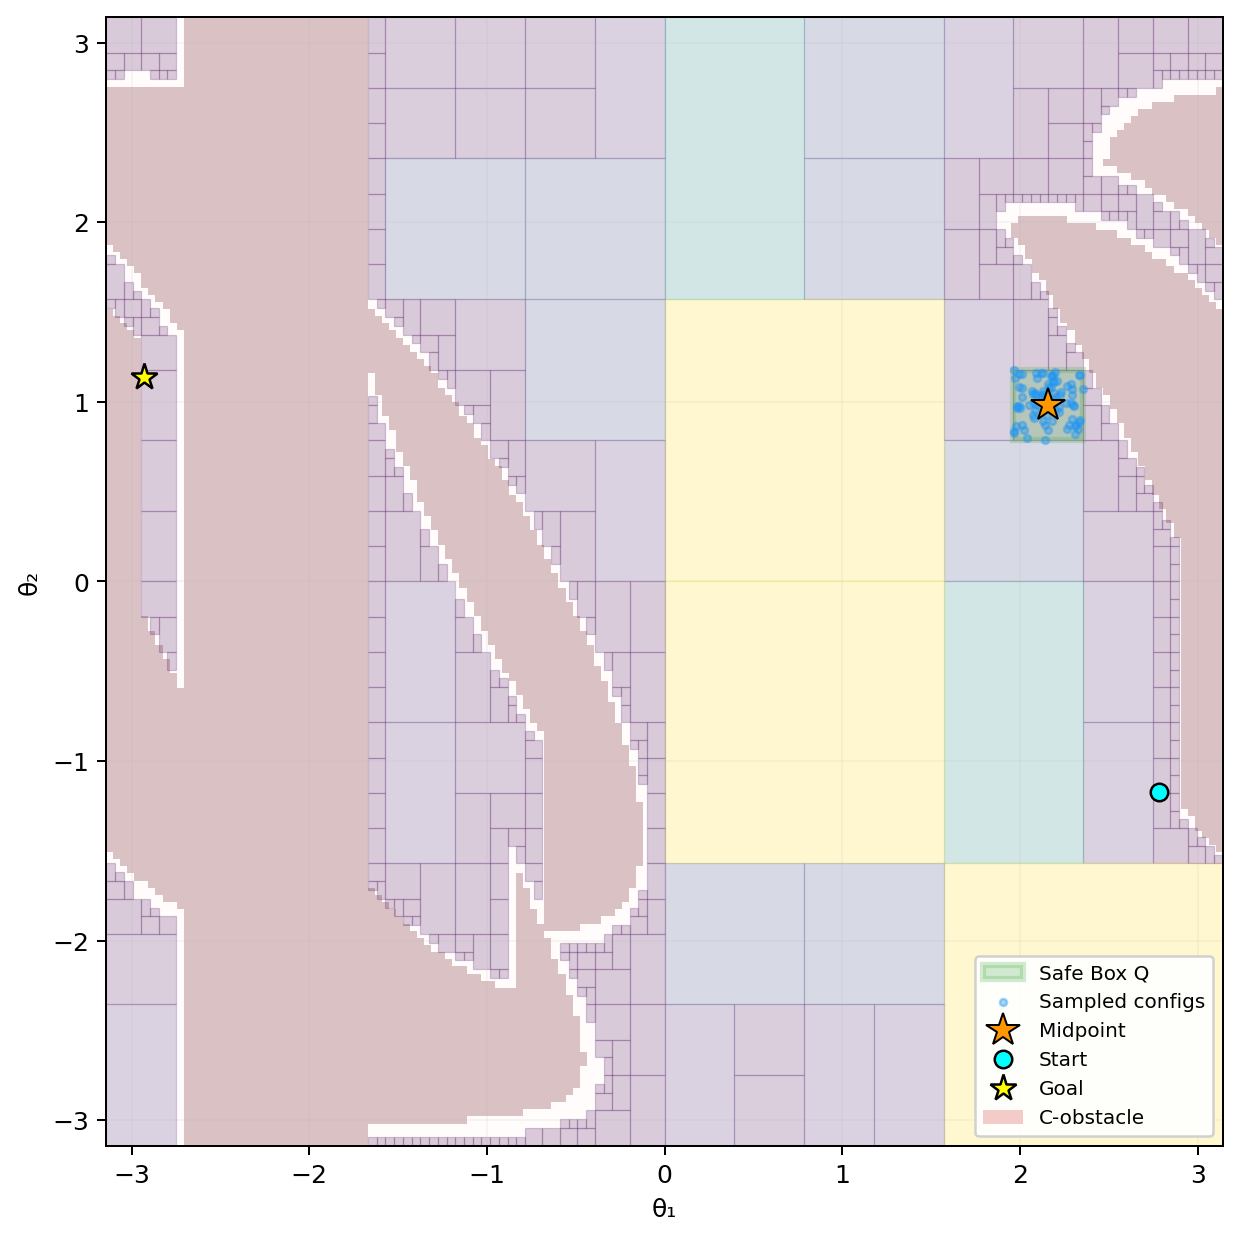
\includegraphics[width=0.325\textwidth]{figures/sbf_grow_1.png} &
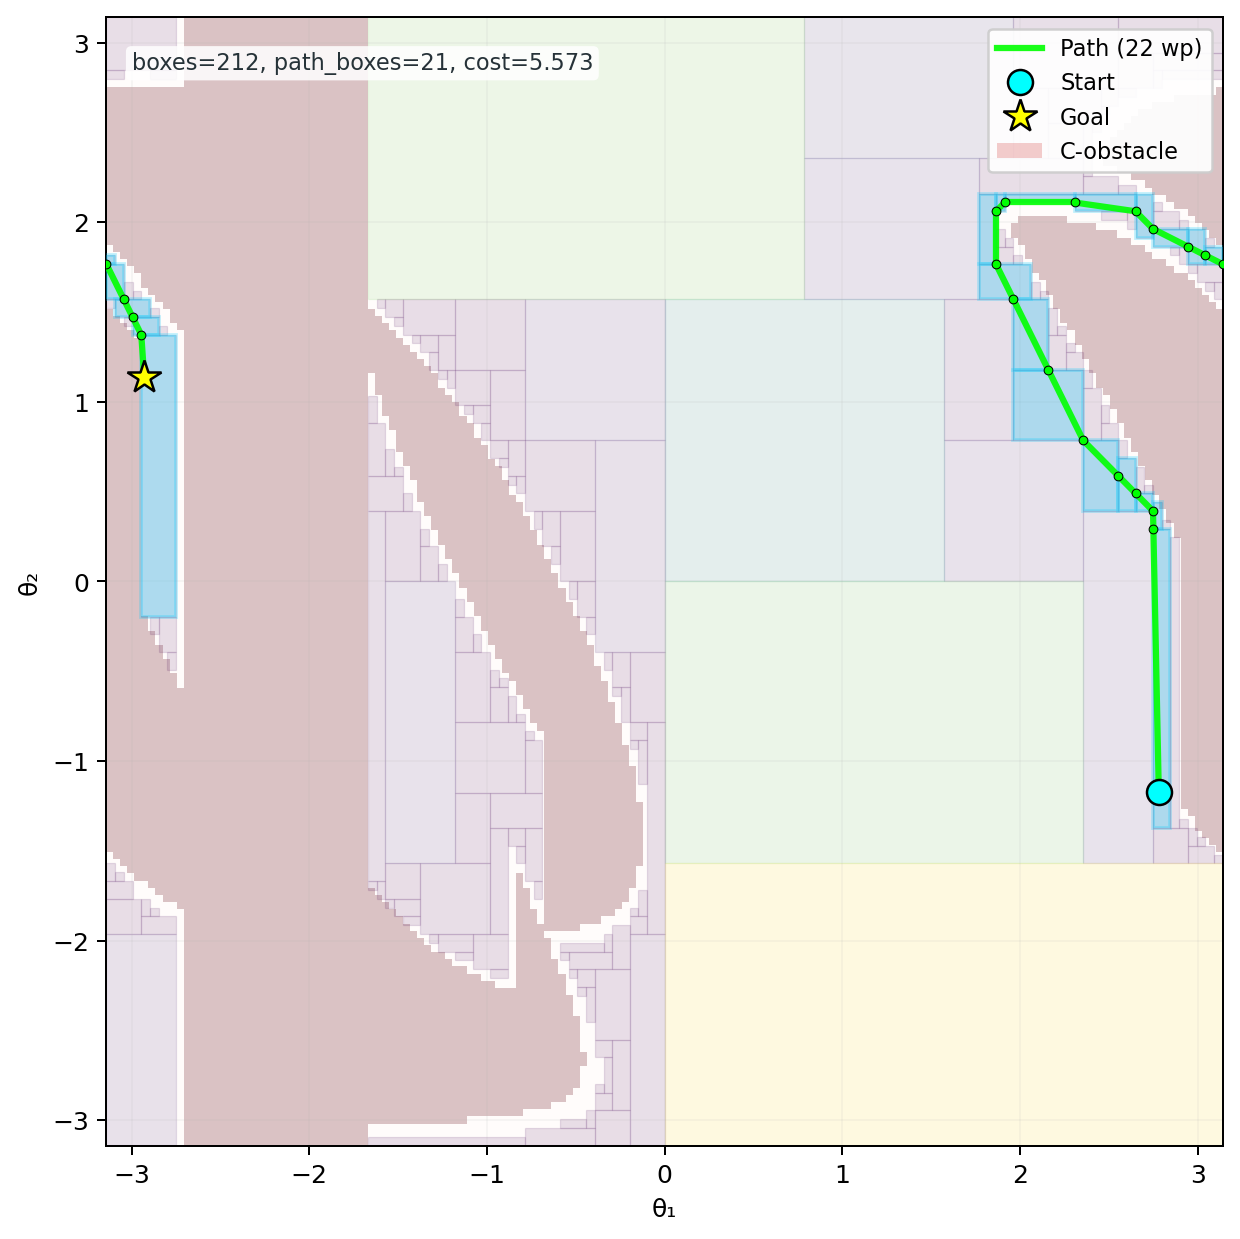
\includegraphics[width=0.325\textwidth]{figures/sbf_grow_3.png} &
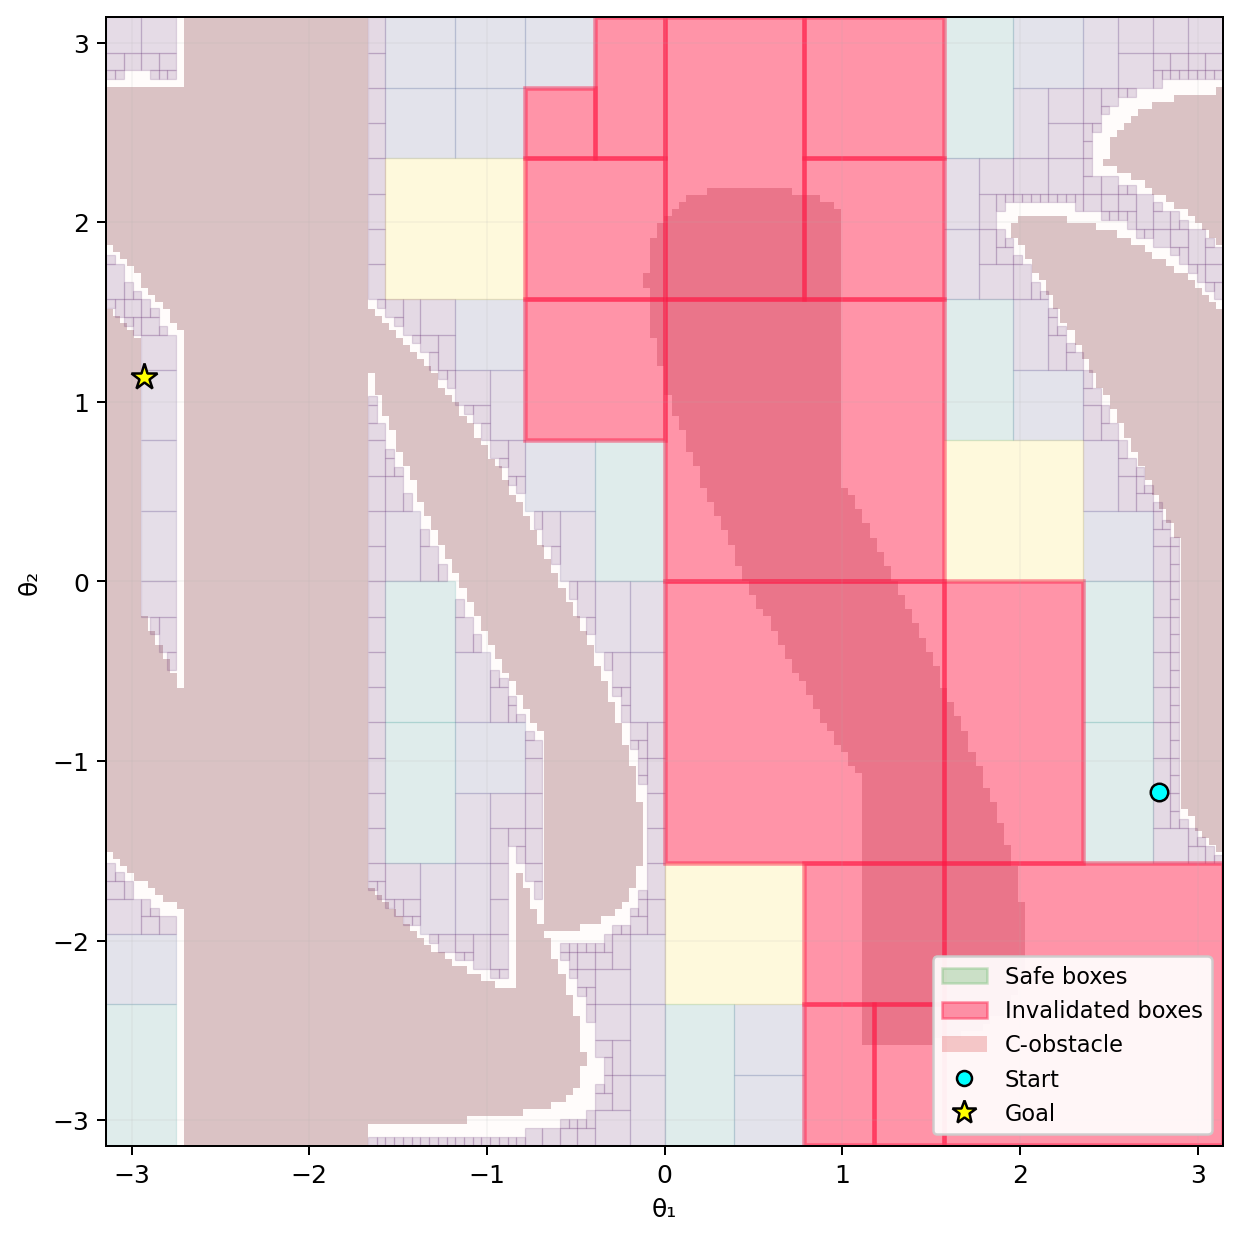
\includegraphics[width=0.325\textwidth]{figures/sbf_grow_5.png} \\
{\footnotesize (a) C-space cells \& box $Q$} &
{\footnotesize (c) C-space path} &
{\footnotesize (e) Invalidated boxes} \\[4pt]
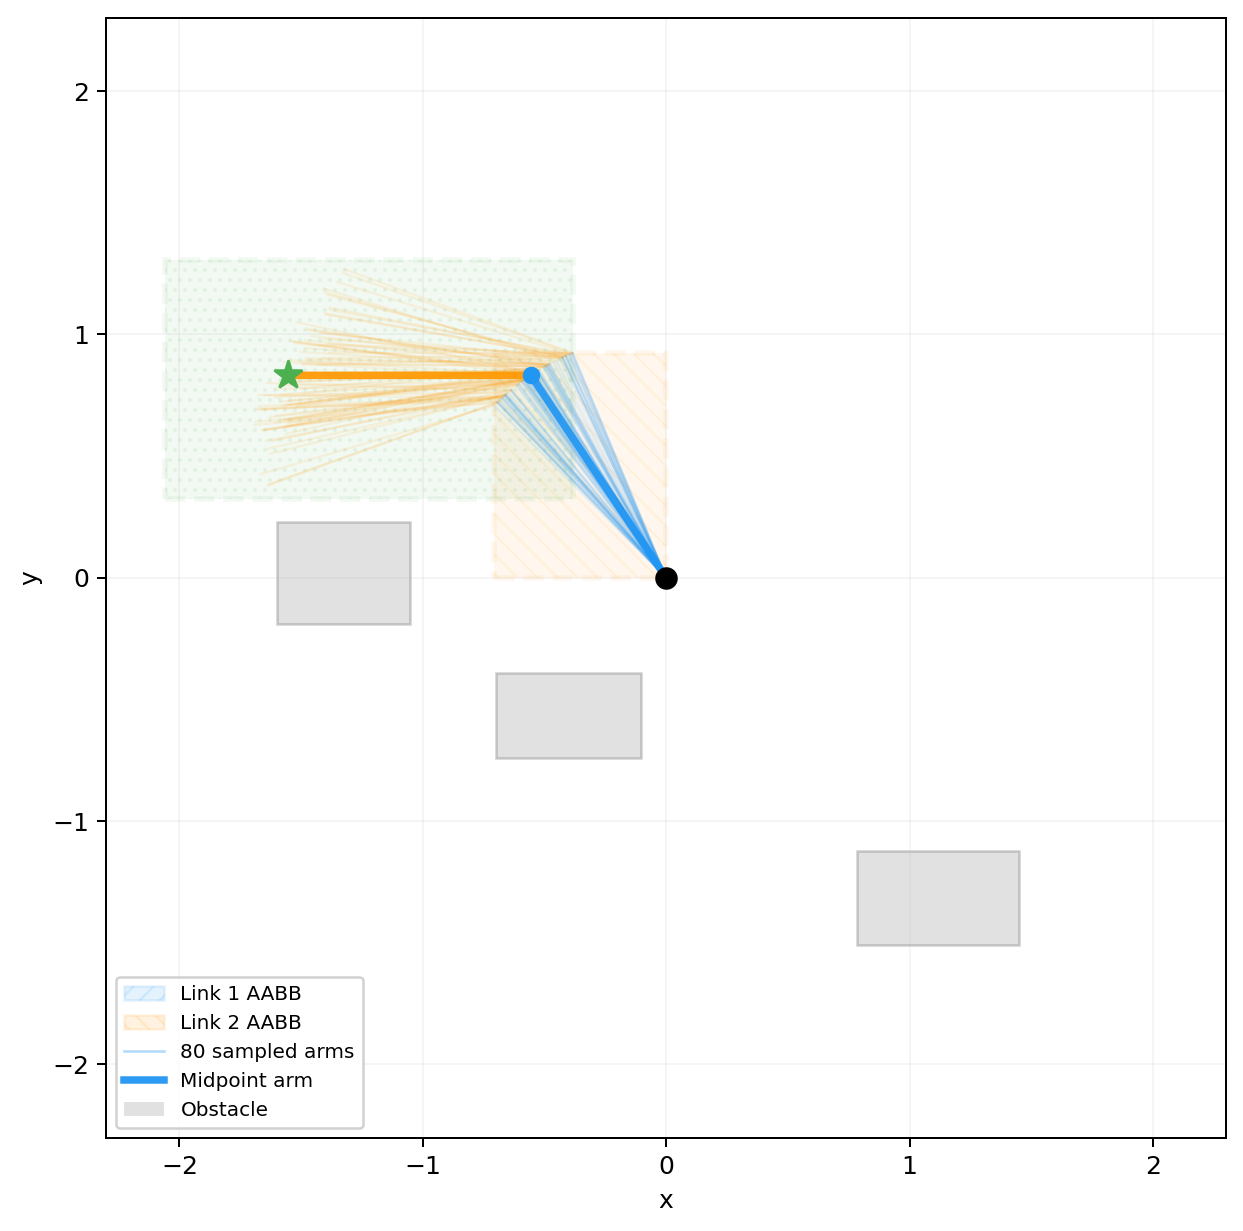
\includegraphics[width=0.325\textwidth]{figures/sbf_grow_2.png} &
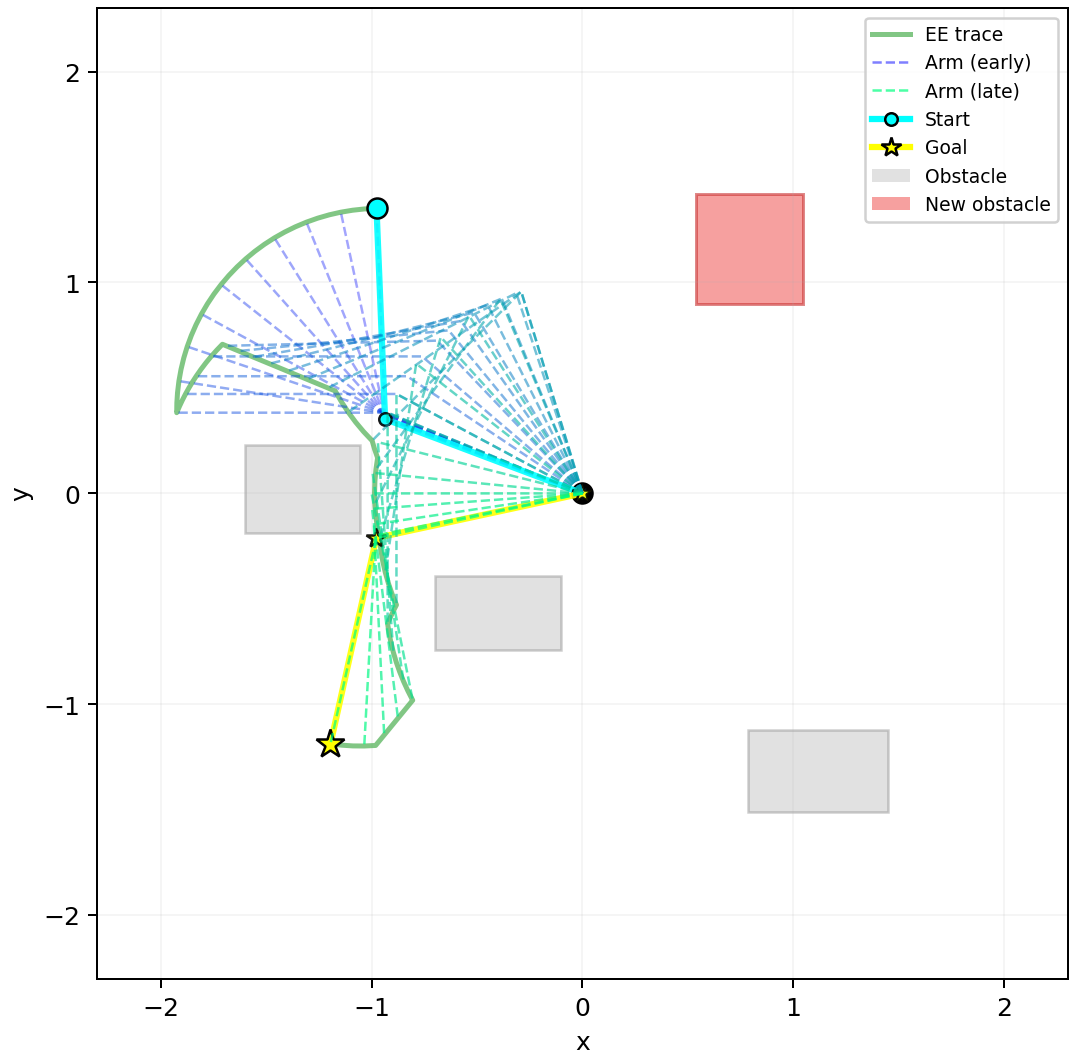
\includegraphics[width=0.325\textwidth]{figures/sbf_grow_4.png} &
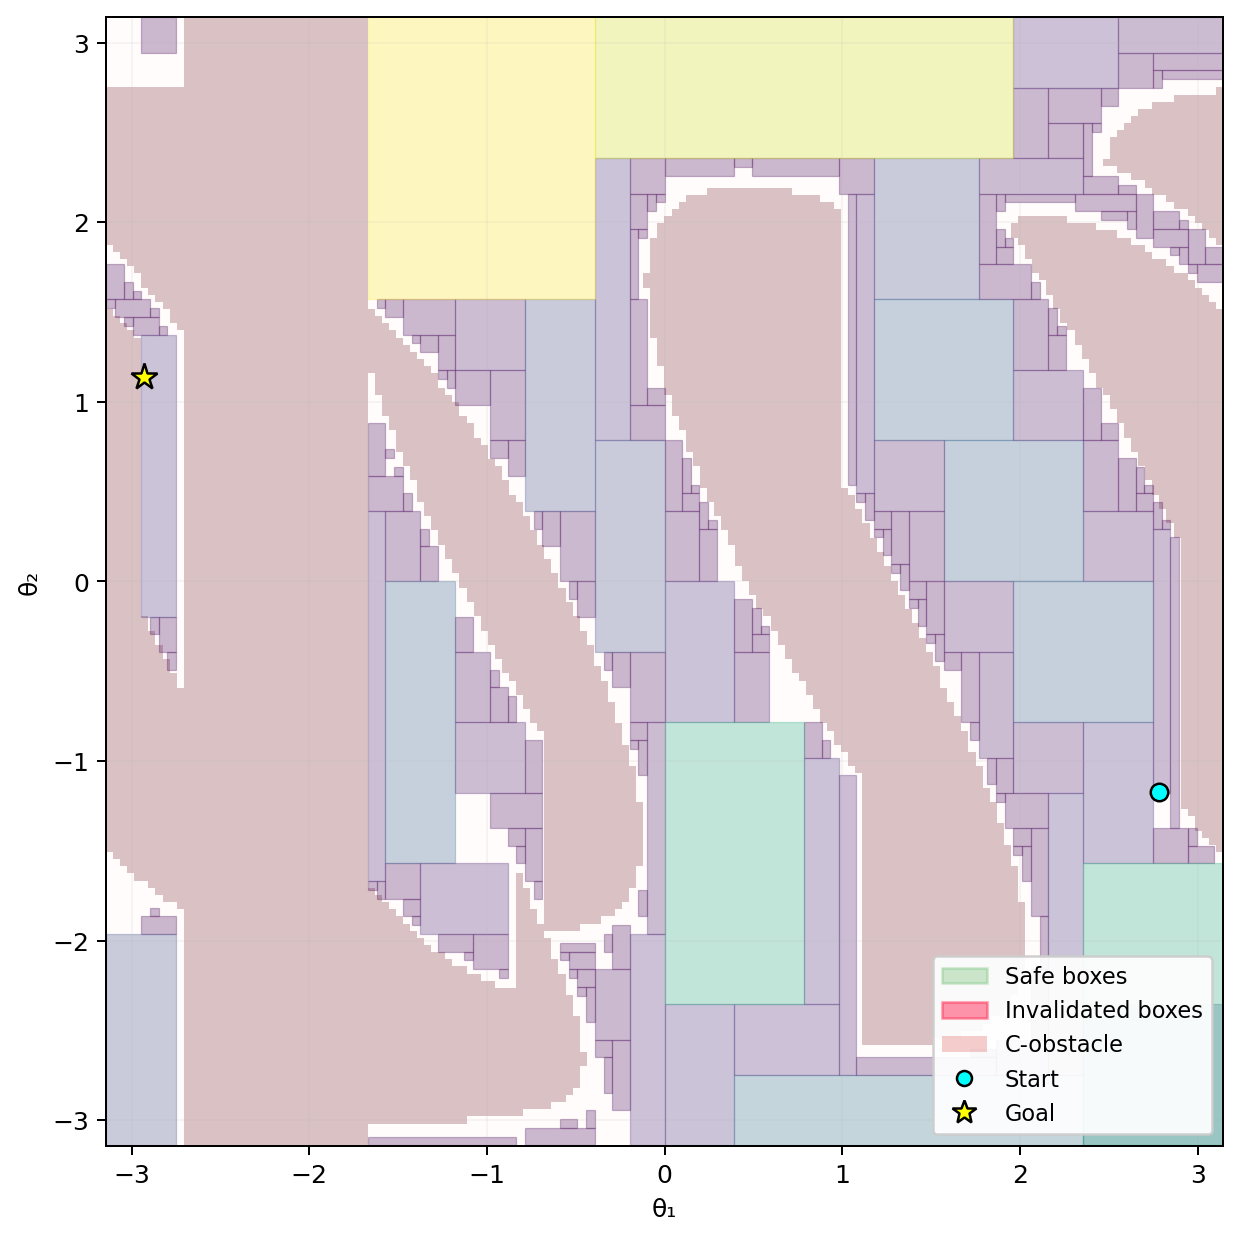
\includegraphics[width=0.325\textwidth]{figures/sbf_grow_6.png} \\
{\footnotesize (b) Workspace AABBs of $Q$} &
{\footnotesize (d) Workspace path} &
{\footnotesize (f) After regrowth} \\
\end{tabular}
\caption{Illustrative \rbf{} build, query, and obstacle-update cycle on a planar 2-link manipulator.
  (a,\,b)~Adaptive $C$-space cells and workspace AABB envelopes of the highlighted box~$Q$.
  (c,\,d)~Box-corridor path in $C$-space and its workspace trajectory.
  (e,\,f)~After obstacle insertion, intersecting boxes are invalidated (red), and localized repair/regrowth updates the explicit forest without requiring a full rebuild.}
\label{fig:overview}
\end{figure*}

This section describes the planning layer of \rbf{}. The algorithm grows a
scene-specific forest of $C$-space boxes and exports the forest as a graph for
repeated corridor queries. The growth loop is RRT-like, but the state added to
the data structure is a free region rather than a point or edge: samples select
frontiers, the link-envelope oracle materializes a usable box, and accepted
boxes extend a connected region graph. In adaptive cell-decomposition language,
the boxes are cells, FindFreeBox is the local refinement and classification
primitive, and the forest graph is the adjacency structure used for query
search. The link interval envelopes of \cref{sec:link_envelopes} and the
optional LECT cache of \cref{sec:lect} serve this planner as collision-filtering
and materialization tools.

Throughout this section, a validated box means a box accepted by the selected
scene-validation policy. In strict conservative mode, paths that remain inside
the validated box union inherit the corridor statement below. In all reported
planning experiments, paths that leave this union through repair, smoothing, or
external composition are charged where used and passed through the same final
scene audit.

Conceptually, the build process has three stages. First, a seed-guided local
oracle adaptively refines and classifies a $C$-space cell around a selected
configuration. Second, repeated frontier expansion grows these cells into a
connected forest, giving the method its region-valued RRT/PRM character. Third,
consolidation coarsens redundant boxes before the structure is exported as a
query graph. The consolidation pass is part of the reusable build phase and its
time is included in reported build measurements.

\subsection{Construction Objective}\label{sec:forest_objective}

Let $\Q$ denote the joint-limit box and let $\calO$ denote the current obstacle
set. The construction objective is to build a finite family
\[
\mathcal{F} = \{B_1,\dots,B_N\}, \qquad B_i \subseteq \Q,
\]
such that every $B_i$ is a validated free-space box, the union
$\bigcup_i B_i$ covers as much useful query-relevant free space as possible
under the available box, time, and depth budgets, and the induced adjacency
graph supports efficient downstream search. This object is scene-specific:
changing $\calO$ changes which intervals are accepted into the forest, even
though the underlying envelope evidence in LECT remains reusable.

The central structural rule is that the forest is not merely a free-space cover,
but a \emph{corridor-compatible} free-space cover. Boxes are inserted
under a connected-box constraint.

Viewed as adaptive cell decomposition, this objective is intentionally
workload-biased rather than globally exhaustive. The planner does not try to
classify every cell in $\Q$. It refines and accepts cells near useful frontiers,
task seeds, and connector candidates, then keeps the resulting adjacency graph
as the reusable planning object.

\paragraph{Connected-box rule.}
For boxes
\[
B_i = \prod_{d=1}^{n}[l_i^{(d)},u_i^{(d)}],
\qquad
B_j = \prod_{d=1}^{n}[l_j^{(d)},u_j^{(d)}],
\]
\rbf{} treats them as connected when, in every coordinate, the two intervals
either overlap or are separated by at most a small tolerance $\varepsilon_c$:
\[
\max\{l_i^{(d)},l_j^{(d)}\}
\le
\min\{u_i^{(d)},u_j^{(d)}\}+\varepsilon_c,
\qquad d=1,\ldots,n.
\]
When $\varepsilon_c=0$, this reduces to ordinary interval intersection or
boundary touching in every dimension. A small positive tolerance absorbs the
boundary offset used by grower seeds and floating-point roundoff.

This rule is deliberately weaker than requiring a full shared face. It treats
overlap, touching, and tolerance-scale gaps uniformly as graph-connectivity
evidence, while validity remains attached to the accepted box union itself. The
output of the construction stage is a forest of validated boxes whose graph
connectivity is aligned with the corridor object queried later, without imposing
a stricter face-sharing invariant than the grower actually maintains.

\subsection{Find Free Box}\label{sec:forest_ffb}

\textsc{FindFreeBox} descends LECT from the root toward the leaf containing
seed $q\in\Q$, materializing endpoint and link envelopes lazily along the path,
skipping saturated subtrees via occupancy metadata, and returning the current
interval as a validated box candidate as soon as the scene oracle accepts it.
Tree topology and endpoint records are reused from the scene-independent cache,
while scene-specific validation is deferred to each grower visit.
\Cref{alg:ffb_rewrite} gives the complete pseudocode.

\begin{algorithm}[t]
\caption{FindFreeBox: local box materialization around a seed.}
\label{alg:ffb_rewrite}
\footnotesize
\begin{algorithmic}[1]
\REQUIRE Seed configuration $q$, LECT $T$, obstacle set $\calO$, depth cap $D_{\max}$
\ENSURE Validated interval $I_v$ or failure
\STATE $v \gets \mathrm{root}(T)$; $d \gets 0$; initialize current interval and FK state
\WHILE{$d \le D_{\max}$}
  \algcommentline{Cache materialization}
  \STATE materialize the endpoint and link envelopes of $v$ if needed
  \algcommentline{Scene validation}
  \IF{$v$ is marked fully occupied}
    \RETURN failure
  \ENDIF
  \IF{$v$ is validated collision-free with respect to $\calO$}
    \RETURN interval $I_v$
  \ENDIF
  \algcommentline{Refinement}
  \IF{$d = D_{\max}$}
    \RETURN failure
  \ENDIF
  \IF{$v$ has no children}
    \STATE split $v$ along the depth-synchronous split dimension of depth $d$
  \ENDIF
  \STATE $k \gets$ split dimension of $v$
  \STATE $v \gets$ the child of $v$ whose interval contains $q$; update the current interval
  \STATE update the FK state from dimension $k$ onward; $d \gets d+1$
\ENDWHILE
\RETURN failure
\end{algorithmic}
\end{algorithm}

The termination behavior is straightforward. Under depth cap $D_{\max}$, each
loop iteration either returns immediately or descends one more level in the
tree, so the procedure can make at most $D_{\max}+1$ decisions. In strict
conservative mode, any returned interval has passed envelope disjointness
against $\calO$; in performance-oriented modes, the returned interval is a
validated planning region that remains subject to the common final audit used
for reported paths.

\subsection{Forest Growth}\label{sec:forest_growth}

Starting from an initial seed set, the forest is grown by repeatedly invoking
the find-free-box procedure on carefully chosen candidate configurations.
Each seed first produces a root box through the find-free-box procedure, and
these root boxes initialize one or more connected components of the forest.
The main grower should be understood as an evidence-guided rapidly exploring
process rather than as a generic random cover: every iteration chooses a
frontier component, proposes a nearby interval worth testing, and accepts the
result only when it extends the forest by a usable connected corridor segment.

Each iteration makes two explicit heuristic decisions: it samples a target
configuration $q_t$, then chooses a boundary seed on an existing box face that
is closest to that target. The reported planning configuration uses a sequential
Bernoulli schedule with component-connector probability $p_c=0.45$, query-root
bias $p_g=0.20$, intertree-root bias $p_i=0.25$, and unexplored-volume
probability $p_u=0.45$. A component-connector target between disconnected root
components is attempted first. If no connector target is used, coordinated
multi-tree mode may target a root from another active component; because
$p_i\le 0.5$ in the reported runs, no high-bias pulse is active and the
sustained cap is also $0.25$. If no intertree target is used, the grower then
tries a query-root target, then a LECT unexplored-volume leaf, and finally a
uniform root-interval sample. The same reported configuration uses 5000 boxes,
a 60~s build timeout, an FFB depth cap of 120, eight worker threads, a
component-connector candidate limit of four, a staged component-connect radius
of 0.35 in normalized $L_\infty$ distance, a post-connect time budget of
450~ms, and a quality floor of 64 connected boxes. These numbers are planner
settings rather than envelope-theory parameters, but they are part of the
self-contained specification for the reported rows.

Given a target $q_t$ and an existing box
$B=\prod_j[\ell_j,u_j]$, the grower enumerates feasible faces
$f=(B,d,s)$, where $d$ is a joint dimension and $s\in\{-1,+1\}$ is the lower or
upper side. Let $\tau$ be the adjacency tolerance and
$\epsilon_b=\max(\epsilon_{\mathrm{guard}},\tau/4)$. A face is feasible only if
stepping outside it by $\epsilon_b$ remains inside the global root interval. In
the reported configurations $\epsilon_{\mathrm{guard}}=0$, so this formula uses
the $\tau/4$ floor. The
seed associated with the face is
\begin{equation}
q_f[j] =
\begin{cases}
u_d+\epsilon_b, & j=d,\ s=+1,\\
\ell_d-\epsilon_b, & j=d,\ s=-1,\\
\operatorname{clip}(q_t[j],\ell_j+\epsilon_b,u_j-\epsilon_b), & j\ne d,
\end{cases}
\end{equation}
with clipping to $[\ell_j,u_j]$ when a box is thinner than $2\epsilon_b$. Faces
are ranked by the squared target distance
\begin{equation}
  \sigma(f;q_t)=\|q_t-q_f\|_2^2,
\end{equation}
and the implementation retains the 128 lowest-score face candidates across the
scanned frontier boxes. It then tries them in increasing score order, skipping a
candidate if the corresponding LECT leaf is temporarily cooled or if a
component-connection cache has already recorded the same boundary seed. The
first remaining candidate becomes the seed for \textsc{FindFreeBox}.

The candidate box is accepted only if \textsc{FindFreeBox} validates it and the
new box is connected to its parent under the same adjacency predicate used by
the query graph: all dimensions overlap up to tolerance $\tau$, and at least one
dimension touches within tolerance or all dimensions overlap. Failures are also
handled explicitly. When the LECT leaf containing a failed seed reaches the
hard-frontier failure threshold of one failed attempt, the leaf is skipped for a
horizon of 300 subsequently accepted boxes, unless a later depth stage raises
the active search depth and enables a retry. Cooling and the frontier-seed cache
do not alter the validation boundary;
they only reduce repeated calls on already failed or already covered frontier
regions. The resulting method is summarized in \cref{alg:forest_growth}.

\begin{algorithm}[t]
\caption{GrowForest: budgeted expansion of a connected box-region forest.}
\label{alg:forest_growth}
\footnotesize
\begin{algorithmic}[1]
\REQUIRE LECT $T$, obstacle set $\calO$, seed set $\mathcal{S}$, box budget $N_{\max}$, time budget $t_{\max}$
\ENSURE Validated box-region forest $\mathcal{F}$
\STATE $\mathcal{F} \gets \emptyset$; initialize connected components from $\mathcal{S}$
\FORALL{$q \in \mathcal{S}$}
  \STATE $B \gets \procname{FindFreeBox}(q, T, \calO)$
  \IF{$B \neq \emptyset$}
    \STATE insert $B$ into $\mathcal{F}$ as a root box
  \ENDIF
\ENDFOR
\WHILE{$|\mathcal{F}| < N_{\max}$ and time budget not exhausted}
  \STATE draw target $q_t$: connector with prob. $p_c$, query/intertree root with prob. $p_g$ or $p_i$, unexplored LECT leaf with prob. $p_u$, otherwise uniform
  \STATE enumerate feasible faces $f=(B,d,s)$ of frontier boxes and compute $q_f$ and $\sigma(f;q_t)$
  \STATE choose the first of the 128 lowest-score face seeds that is not cooled and not in the frontier-seed cache
  \STATE set $(q_{\mathrm{seed}},B_{\mathrm{near}}) \gets (q_f,B)$ for that face
  \STATE $B_{\mathrm{new}} \gets \procname{FindFreeBox}(q_{\mathrm{seed}}, T, \calO)$
  \IF{$B_{\mathrm{new}} \neq \emptyset$ and $\procname{BoxesConnected}(B_{\mathrm{new}},B_{\mathrm{near}},\tau)$}
    \STATE insert $B_{\mathrm{new}}$ into $\mathcal{F}$; $\procname{UpdateComponents}(\mathcal{F})$
  \ELSE
    \STATE record the failed LECT leaf; cool it after one failed attempt for a 300-box horizon
  \ENDIF
\ENDWHILE
\RETURN $\mathcal{F}$
\end{algorithmic}
\end{algorithm}

The main reported configuration uses coordinated multi-goal growth. Five seed
configurations initialize the shelf roots, and the grower uses the fixed
resource budget reported in
\cref{sec:exp_shelf_iiwa,fig:tro_shelf_anytime_tradeoff}. This choice keeps the
growth schedule simple enough to preserve one authoritative forest state while
still exposing reusable LECT evidence across threads and cache-warm reruns.
Staged wavefront growth and task-batched multi-threaded growth are treated as
engineering variants, and the parallel-scaling experiment reports the present
limit of the task-batched variant. The output of this section is the
query-ready box-region object only.

\subsection{Forest Consolidation}\label{sec:forest_consolidation}

Raw growth tends to produce a forest that is finer than necessary. The purpose
of consolidation is to replace a large collection of locally valid
boxes by a smaller collection of equally valid but more useful regions.
Two operations are central.

The first is \emph{promotion}. When two occupied sibling leaves are both
collision-free and their parent interval is also collision-free, the two leaves can be
replaced by the parent. This is the most local form of coarsening and directly
reuses the multiresolution structure of LECT.

The second is \emph{multi-level coarsening}. Exact connected merges are the
cleanest case: if two boxes are connected and their union is itself one box,
the merged region can be accepted directly after validation. More general
connected candidate merges are handled by constructing a candidate parent
region and accepting it only when its chosen envelope representation remains
collision-free against the current obstacle set. This is where the representation choices of
\Cref{sec:link_envelopes,sec:lect} become operational. In an AABB-based forest, the compact parent witness
is typically the enclosing AABB of the two child boxes. KDOP parents can merge
child slab intervals by per-axis minima and maxima, while SupportHull parents
are kept compact only when the merged endpoint-hull witness remains acceptable;
otherwise the child witnesses are retained. Greedy non-sibling candidates are
ranked by a volume-expansion score, so exact face merges are preferred and
high-inflation parents are deferred unless they pass validation under the
scene oracle. The consolidation logic is summarized in
\Cref{alg:forest_consolidation}.
The final containment-pruning step removes only boxes that are fully covered by
accepted validated regions and whose graph incidence can be transferred to a
retained covering region. It changes neither the represented
free-space union nor the corridor witnesses used by query search.

\begin{algorithm}[t]
\caption{ConsolidateForest: graph-preserving promotion, merging, and pruning.}
\label{alg:forest_consolidation}
\footnotesize
\begin{algorithmic}[1]
\REQUIRE Validated forest $\mathcal{F}$, LECT $T$, obstacle set $\calO$
\ENSURE Consolidated validated forest $\mathcal{F}'$
\STATE $\mathcal{F}' \gets \mathcal{F}$
\algcommentline{Stage 1: sibling promotion}
\REPEAT
  \STATE promote any validated sibling leaves whose parent is collision-free
\UNTIL{no eligible sibling pair remains}
\algcommentline{Stage 2: validated connected/contact merging}
\STATE merge exact connected pairs whose union is itself a single box
\FORALL{connected candidate pairs $(B_i,B_j)$ in $\mathcal{F}'$}
  \STATE build a candidate parent region $H$ and score its volume expansion
  \IF{the chosen envelope representation of $H$ is collision-free with respect to $\calO$}
    \STATE replace $B_i,B_j$ by $H$
  \ENDIF
\ENDFOR
\algcommentline{Stage 3: containment pruning}
\STATE remove only contained boxes whose adjacency and segment witnesses transfer to retained covering regions
\RETURN $\mathcal{F}'$
\end{algorithmic}
\end{algorithm}

Validity follows directly: every accepted promotion or merge has itself passed
the scene oracle, so the represented free-space union cannot shrink.
Containment pruning removes only boxes fully covered by a retained region that
inherits their adjacency witnesses, preserving all corridor connectivity.

\subsection{Corridor Query}
\label{sec:forest_graph}

After growth and consolidation, the forest is exported as a graph
$G=(V,E)$ with one vertex per validated box. Two vertices are connected by an
edge when their boxes satisfy the connected-box rule above. Lightweight querying is possible because this
connected-box structure is enforced during growth and consolidation rather
than repaired after graph export.

If disconnected adjacency islands remain after growth, an optional connector
stage attempts targeted bidirectional sampling bridges between nearest frontier boxes
of different components. A successful bridge is stored as a segment edge rather
than as a claim that the two boxes overlap. This distinction is important for
both the \rbf{} query layer and the GCS negative controls: a segment edge is a
collision-checked path witness between two boxes, whereas a GCS edge over
convex regions requires feasible overlap of the regions themselves.

This pair $(\mathcal{F},G)$ is the final planning object produced by the build
stage. Querying it is intentionally lightweight. Given start and goal
configurations $q_s,q_g$, the planner associates them with start-side and
goal-side boxes in $\mathcal{F}$ and then searches $G$ for a connecting box
sequence. The query problem is reduced to box-corridor
retrieval inside an already constructed free-space representation.

A shortest path on $G$ yields a box sequence whose union defines a corridor
between the two query endpoints. A geometric path is then recovered as a
waypoint chain inside that corridor. In the experiments, this candidate is then
passed through the same OMPL-style simplification/local post-processing and
fixed-step final audit used by the comparison pipelines. That post-processing
can move the final reported path outside the source box union. Consequently,
the box-corridor statement below applies only to contained paths before or after
post-processing, while the reported planning success in the main curves is the
common fixed-resolution audit outcome.

\begin{theorem}[Conditional validated box-corridor path]
\label{thm:corridor_certificate}
Let $\mathcal{F}$ be a forest whose boxes have each passed conservative
link-envelope validation against obstacle set $\calO$. If a continuous path
$\gamma:[0,1]\to\Q$ satisfies
$\gamma([0,1])\subseteq \bigcup_{B\in\mathcal{F}}B$, then every configuration
on $\gamma$ is collision-free with respect to $\calO$.
\end{theorem}

\begin{proof}
For any $s\in[0,1]$, the containment assumption gives a validated box
$B\in\mathcal{F}$ with $\gamma(s)\in B$. By construction, validation of $B$
means every conservative link envelope for $B$ is disjoint from $\calO$.
Because each such envelope contains the link geometry for every configuration
inside $B$ (\cref{sec:link_envelopes}), the robot geometry at $\gamma(s)$ is
also disjoint from $\calO$. Since $s$ was arbitrary, the whole path is
collision-free.
\end{proof}

\paragraph{Reporting protocol.}
\Cref{thm:corridor_certificate} is a conditional statement: it covers path
portions contained in a conservatively validated box union. It is not the
acceptance rule for the main experimental comparisons. When OMPL simplification,
local repair, smoothing, or external composition leaves that union, the path is
accepted only if it passes the same fixed-resolution final scene collision audit
used for the baselines. The main performance curves should therefore be read as
post-processed, fixed-audit planning results rather than as evidence that every
reported path satisfies the box-corridor containment hypothesis.

For dynamic scenes, the same explicit forest representation supports local
graph maintenance without compulsory rebuilds. Each accepted box records the
obstacle evidence that blocked or validated its envelope tests; obstacle
deletions cannot invalidate existing boxes accepted under the same validation
policy, because free space only grows. Deletion triggers only a spatial dirty-region pass around the removed
obstacle to choose local regrowth seeds, after which any new box is validated by
the same oracle as in the original build. Obstacle insertion is stricter: the
new obstacle is inflated by the dirty-region padding, all overlapping boxes are
rechecked exactly, invalid boxes and incident graph edges are removed, and every
surviving segment edge is re-audited in the edited scene. The repair stage then
regrows from deleted-box centers, live neighbours, original task seeds, and
component-boundary candidates; each committed box must pass the active
validation policy before it enters the forest. Finally, query failure can trigger a
bounded local repair search, again filtered by the same final audit. Warm
rebuild remains available as a measured baseline and fallback policy.

% \begin{algorithm}[t]
% \caption{\textsc{IncrementalUpdate}---localized certificate invalidation and graph repair}
% \label{alg:incremental_update}
% \footnotesize
% \begin{algorithmic}[1]
% \REQUIRE Conservative forest $\mathcal{F}$, graph $G$, edited obstacles $\Delta\calO$, LECT $T$
% \ENSURE Repaired forest and adjacency graph, or failure
% \STATE $\mathcal{I} \gets \emptyset$
% \FORALL{$B \in \mathcal{F}$}
%   \IF{the link envelope of $B$ intersects any obstacle in $\Delta\calO$}
%     \STATE add $B$ to invalidated set $\mathcal{I}$
%   \ENDIF
% \ENDFOR
% \STATE remove $\mathcal{I}$ from $\mathcal{F}$ and delete incident graph edges from $G$
% \STATE rebuild connected-box edges among surviving neighbouring boxes
% \IF{localized regrowth is enabled}
%   \STATE seed \textsc{GrowForest} near frontier boxes adjacent to removed regions
%   \STATE accept only boxes conservatively collision-free under the edited scene
% \ENDIF
% \STATE \textbf{return} repaired $(\mathcal{F},G)$ if queried components remain connected; otherwise failure
% \end{algorithmic}
% \end{algorithm}

If no contained conservative corridor is recovered, no box-corridor guarantee
attaches to that query. The construction still exports a concrete box-region
planning object, and \cref{sec:exp} evaluates its build cost, query cost, path
quality, and success rate after the same post-processing and fixed-resolution
final audit used for the other planners.

\section{Experiments}\label{sec:exp}

This section evaluates \rbf{} as a multi-query planning system whose returned
paths are compared after common post-processing and fixed-resolution final
audit. The primary question is the design point:
how much reusable build/query time can the implemented \rbf{} pipeline save on
the tested workloads, and what audited path-length gap does it pay? The
endpoint/link envelope, LECT, and dynamic-update studies explain construction
cost and maintenance behavior within the same scoped system evaluation.

\paragraph{Scope.}
The main evidence consists of the Shelf+IIWA and IIWA/UR5/Panda anytime
trade-off figures with accompanying compact summary tables. Mechanism results
report endpoint interval-AABB behavior, the CritSample-based envelope
representation trade-off, incremental IIWA LECT reuse, and a dynamic-update
capability comparison. Together these experiments support a controlled workload
claim about planning throughput, audited path quality, repeated-query
amortization, and mechanism-level costs. They do not establish distributional
generalization or sensitivity to random seed count, audit resolution, worker
count, row-selection rule, grower strategy, or narrow clearance.

\paragraph{Reporting Protocol.}
The paper uses two reported success notions and one theorem boundary.
\emph{Candidate success} means that a planner produced a candidate path under
its own construction rules; it is a search/solver-completion statistic and is
not credited as safe motion. \emph{Final-audited success} is the common reported
planning metric for all methods: after the method-specific construction and the
shared OMPL-style simplification/local post-processing, every returned path is
checked by the same scene collision oracle at a fixed 0.01 joint-space segment
step. This is a uniform empirical safety check at the stated resolution, not a
continuous certificate. The conservative box-corridor theorem is a narrower
boundary for \rbf{} paths that both use conservative validation and remain
inside the validated box union. It is not used as the acceptance criterion for
the main curves, because the common post-processing, bridge repair, smoothing,
and external composition can leave that union. The
paper-wide audit accounting accepts 663/668 counted paths. The five counted
failures come from the direct merger+GCS negative-control rows in the accounting
suite and are not credited as planning successes; unsafe solved GCS attempts
that are rejected before fallback are tracked separately. A closure scan of the
current artifacts found no stored corridor-containment fields, so the main
planning tables report fixed-resolution final-audited rows only and do not
measure the fraction of those rows that would also stay inside the validated
box union. We also re-audited 3240 stored random-scene
checkpoint paths at several segment steps. The stated 0.01 audit step produced
0 invalid records. Finer checks exposed resolution sensitivity shared by the
pipelines: 0.005 and 0.002 steps found 502 and 678 invalid checkpoint records,
respectively, corresponding to 79 and 111 unique stored paths. Thus the reported
success statistics should be read exactly as fixed-resolution final-audit
statistics, not as continuous safety guarantees or guarantees that the
post-processed path remains inside the box union.

\paragraph{Platform and Scenes.}
All experiments reported here run on an Intel Core i5-12600KF workstation with
16 logical CPUs and 31~GiB RAM. Unless the study itself is the parallel-scaling
sweep, all planners use eight worker threads. Shelf+IIWA uses one canonical
scene with five task pairs and manually selected reference anchors from the
Marcucci scene. The random-scene study spans IIWA/UR5/Panda easy,
medium, and hard settings with 50 fixed random scene seeds per setting, where
easy/medium/hard denote incrementally generated 4/8/12-obstacle scenes. These
counts support a controlled system comparison, but they do not by themselves
establish broad distribution-level generalization.

\paragraph{Baseline Accounting and Seed Policy.}
IRIS-NP+GCS uses the Drake implementation and charges region build. PRM,
RRTConnect, and BIT* use OMPL. We separate reusable multi-query pipelines
(\rbf{}, PRM, IRIS-NP+GCS) from no-build single-query references (RRTConnect
and BIT*): PRM charges roadmap build, IRIS-NP+GCS charges convex-region build,
and \rbf{} charges box-forest build, while RRTConnect and BIT* are treated as
single-query references. RRTConnect uses one
maximum-timeout call per seed/query with no restart accounting and stops on
first connection; a timeout is a failure. BIT* uses one fixed-timeout call per
seed/query, and the plotted curve/table rows are taken from the audited monotone
incumbent checkpoint trace rather than raw checkpoint stage values. The IRIS
comparison should be read as a comparison of the implemented pipelines under a
shared workload-level seed protocol. In the Shelf+IIWA workload, all planners
use the same task pairs and the same manually selected Marcucci reference
anchors, with query-derived midpoint seeds when a planner requires additional
initial points. In the random-scene workload, all planners use the same fixed
random scene/query seeds. This common seed protocol improves baseline fairness,
but the build-time gaps remain full-pipeline results because the region
representations, graph construction, repair, and solver implementations differ.

\paragraph{Acceptance Boundary.}
The main comparison accepts paths by the same fixed-resolution final audit for
all methods. Paths inside conservatively validated \rbf{} corridors inherit the
box-corridor statement, but the shared post-processing step can move a returned
path outside that union. Such paths have only the common final-audit semantics,
so the theorem is not transferred to the main curves.

\paragraph{Tabulated Rows and Omitted Sensitivities.}
Where a table accompanies an anytime figure, the table gives a compact numeric
slice of the corresponding curve rather than a separate evaluation. The
tabulated-row extraction was postprocessed over 820 anytime stage points. The
reported rows were unchanged when the path-tolerance rule was varied over
5\%, 8\%, 10\%, and 15\%; a zero-tolerance shortest-path-only rule changed
25/50 scenario-method rows. At the reported rows, the RBF-SH path gap to the
shortest tabulated method has median 0.056~rad, 90th percentile 0.296~rad, and
maximum 0.455~rad on Shelf+IIWA. These checks support the use of the tables as
compact numeric slices, while the full curves remain the primary evidence.
The present paper still does not exhaustively characterize sensitivity to seed
count, worker count, grower strategy, narrow clearance, or broader audit rules.

\subsection{Shelf+IIWA Efficiency and Path Quality}\label{sec:exp_shelf_iiwa}

\begin{figure*}[t]
  \centering
  \IfFileExists{generated/fig_tro_shelf_anytime_tradeoff_clean.png}{%
    \begin{minipage}[t]{0.75\textwidth}
      \centering
      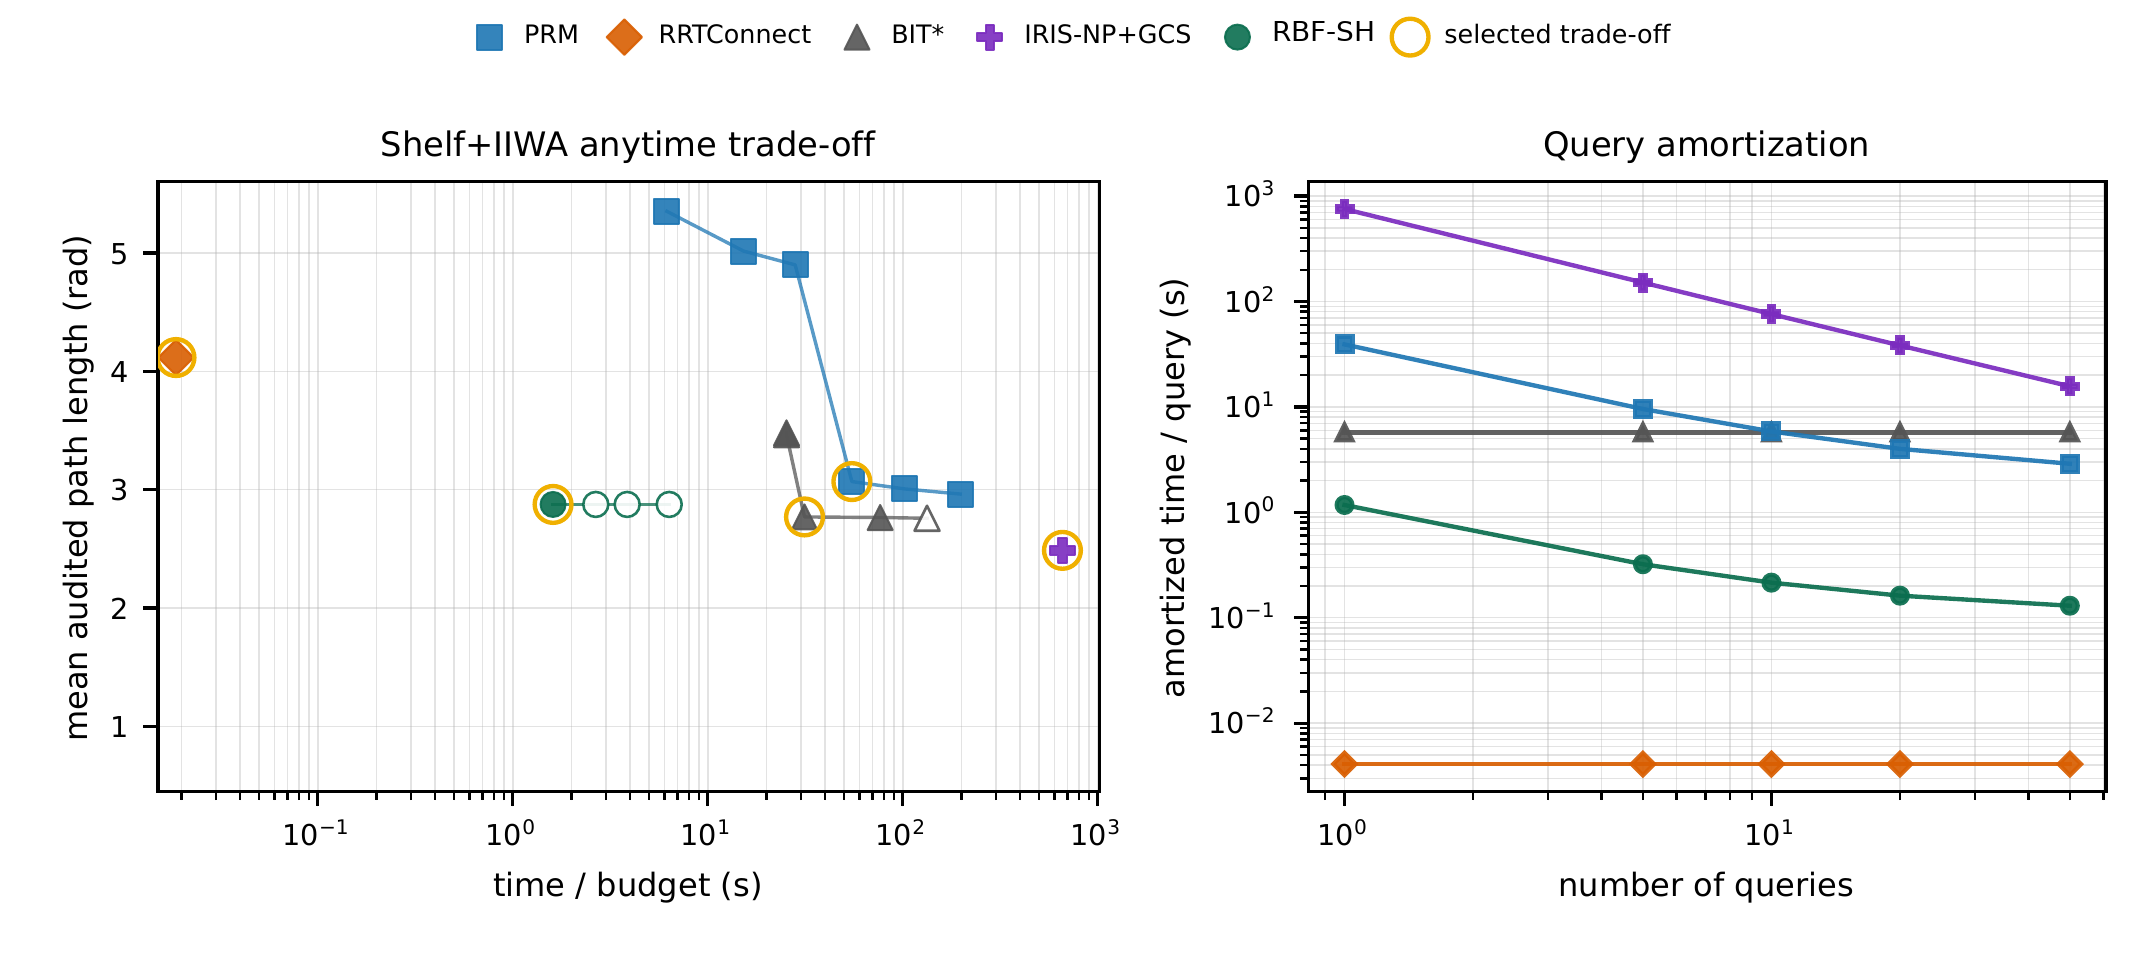
\includegraphics[width=\textwidth]{generated/fig_tro_shelf_anytime_tradeoff_clean.png}%
    \end{minipage}\hfill
    \begin{minipage}[t]{0.24\textwidth}
      \centering
      \raisebox{2.5em}[0pt][0pt]{%
        \IfFileExists{figures/Marcucci_scene.png}{%
          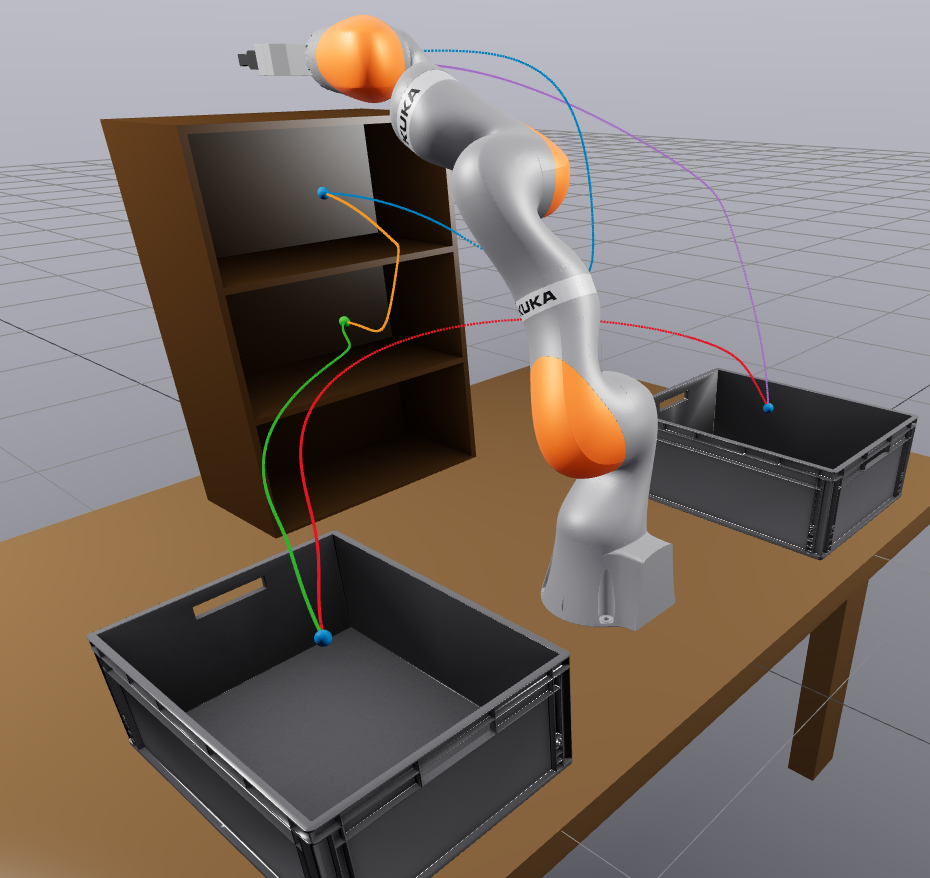
\includegraphics[width=\textwidth]{figures/Marcucci_scene.png}%
      }{%
          \fbox{\parbox{0.95\textwidth}{\centering
          Missing Marcucci_scene.png.}}%
        }%
      }%
    \end{minipage}

    \vspace{-0.45em}
    \begin{minipage}[t]{0.75\textwidth}
      \centering
      \makebox[0.485\linewidth][c]{\footnotesize\textbf{(a)}}%
      \makebox[0.485\linewidth][c]{\footnotesize\textbf{(b)}}
    \end{minipage}\hfill
    \begin{minipage}[t]{0.24\textwidth}
      \centering
      \raisebox{0.35em}[0pt][0pt]{\footnotesize\textbf{(c)}}
    \end{minipage}
  }{%
    \fbox{\parbox{0.92\textwidth}{\centering
    \vspace{0.7em}
    Missing the Shelf+IIWA anytime-tradeoff figure asset.\\
    Regenerate the figure before compiling the manuscript.
    \vspace{0.7em}}}%
  }
  \caption{Shelf+IIWA final-audited design-point trade-off. (a) Anytime trade-off under the method-specific build/query protocol; points nearer the lower-left corner combine lower charged time with shorter audited path length. Filled markers indicate incumbent-improving checkpoints; open markers show a sparse representative subset of nonimproving checkpoints. (b) Amortized per-query cost for the tabulated rows. (c) Canonical Marcucci scene used for the Shelf+IIWA experiments. Gold rings mark the rows reported in \cref{tab:tro_main_shelf_best_tradeoff}. AS, TS, CS, LB, and RB denote the above-shelf target, top shelf, middle shelf, left bin, and right bin, respectively.}
  \label{fig:tro_shelf_anytime_tradeoff}
  \vspace{1em}
  % Auto-generated from current anytime trade-off artifacts.
\begingroup
\centering
\captionof{table}{Common-rule tabulated Shelf+IIWA rows from Fig.~\ref{fig:tro_shelf_anytime_tradeoff}, reported by query. Gold rings in Fig.~4 mark these rows only to expose detailed numeric values; the full curves remain the primary evidence. RRTConnect uses one max-timeout attempt per seed/query and returns on connection; BIT* uses one fixed-timeout invocation per seed/query with an audited monotone incumbent checkpoint trace. OMPL planning, final simplify, and fixed-resolution final audit use the same 0.01 joint-space segment step. Query and path entries are success-only averages over paths that pass this fixed-resolution audit.}
\label{tab:tro_main_shelf_best_tradeoff}
\footnotesize
\setlength{\tabcolsep}{1.55pt}
\renewcommand{\arraystretch}{0.96}
\begin{tabular}{@{}lrr|rr|rr|rr|rr@{}}
\toprule
  & \multicolumn{2}{c}{\textbf{\footnotesize \shortstack{SBF-SH}}} & \multicolumn{2}{c}{\textbf{\footnotesize \shortstack{IRIS-NP+GCS}}} & \multicolumn{2}{c}{\textbf{\footnotesize \shortstack{PRM}}} & \multicolumn{2}{c}{\textbf{\footnotesize \shortstack{RRTConnect}}} & \multicolumn{2}{c}{\textbf{\footnotesize \shortstack{BIT*}}} \\
\cmidrule(lr){2-3}\cmidrule(lr){4-5}\cmidrule(lr){6-7}\cmidrule(lr){8-9}\cmidrule(lr){10-11}
Query & Query (s) & Path & Query (s) & Path & Query (s) & Path & Query (s) & Path & Query (s) & Path \\
\midrule
AS$\rightarrow$TS & -- & -- & -- & -- & -- & -- & -- & -- & -- & -- \\
TS$\rightarrow$CS & -- & -- & -- & -- & -- & -- & -- & -- & -- & -- \\
CS$\rightarrow$LB & -- & -- & -- & -- & -- & -- & -- & -- & -- & -- \\
LB$\rightarrow$RB & -- & -- & -- & -- & -- & -- & -- & -- & -- & -- \\
RB$\rightarrow$AS & -- & -- & -- & -- & -- & -- & -- & -- & -- & -- \\
\bottomrule
\end{tabular}
\par\endgroup

\end{figure*}

\Cref{fig:tro_shelf_anytime_tradeoff} compares Shelf+IIWA anytime incumbents
on the canonical Marcucci workload and shows the corresponding amortization
view. This figure is the first main planning result: it tests whether the
box-region forest reaches a low charged-time design point and what path-length
premium it pays.
All methods in this figure are compared after the common final-path
post-processing and fixed 0.01 joint-space audit protocol; OMPL planners use
the same segment step for planning and final simplify. RRTConnect uses one
maximum-timeout call for each seed/query and exits as soon as a connection is
found. BIT* uses one fixed-timeout call per seed/query, and the plotted line is
the audited monotone incumbent summary across checkpoints rather than raw
checkpoint-stage values. Filled markers denote incumbent-improving checkpoints,
while open markers show only a sparse representative subset of nonimproving
checkpoints. Panel (a) shows the anytime trade-off, panel (b) reports
amortized per-query cost for the tabulated rows, and
\cref{tab:tro_main_shelf_best_tradeoff} gives the corresponding success-only
averages over final-audited trials. In the tabulated Shelf+IIWA slice, RBF-SH
uses a 1.07~s reusable build and sub-0.102~s online queries, but its audited
paths are longer than the IRIS-NP+GCS paths for all five listed queries and are
not uniformly shorter than the BIT* incumbents. The Shelf result should
therefore be read as a latency/amortization trade-off, not as a shortest-path
claim.

\subsection{Balanced Random-Scene Pipeline Study}\label{sec:exp_generalization}

\begin{figure*}[t]
  \centering
  \IfFileExists{generated/fig_tro_random_anytime_tradeoff_clean.png}{%
    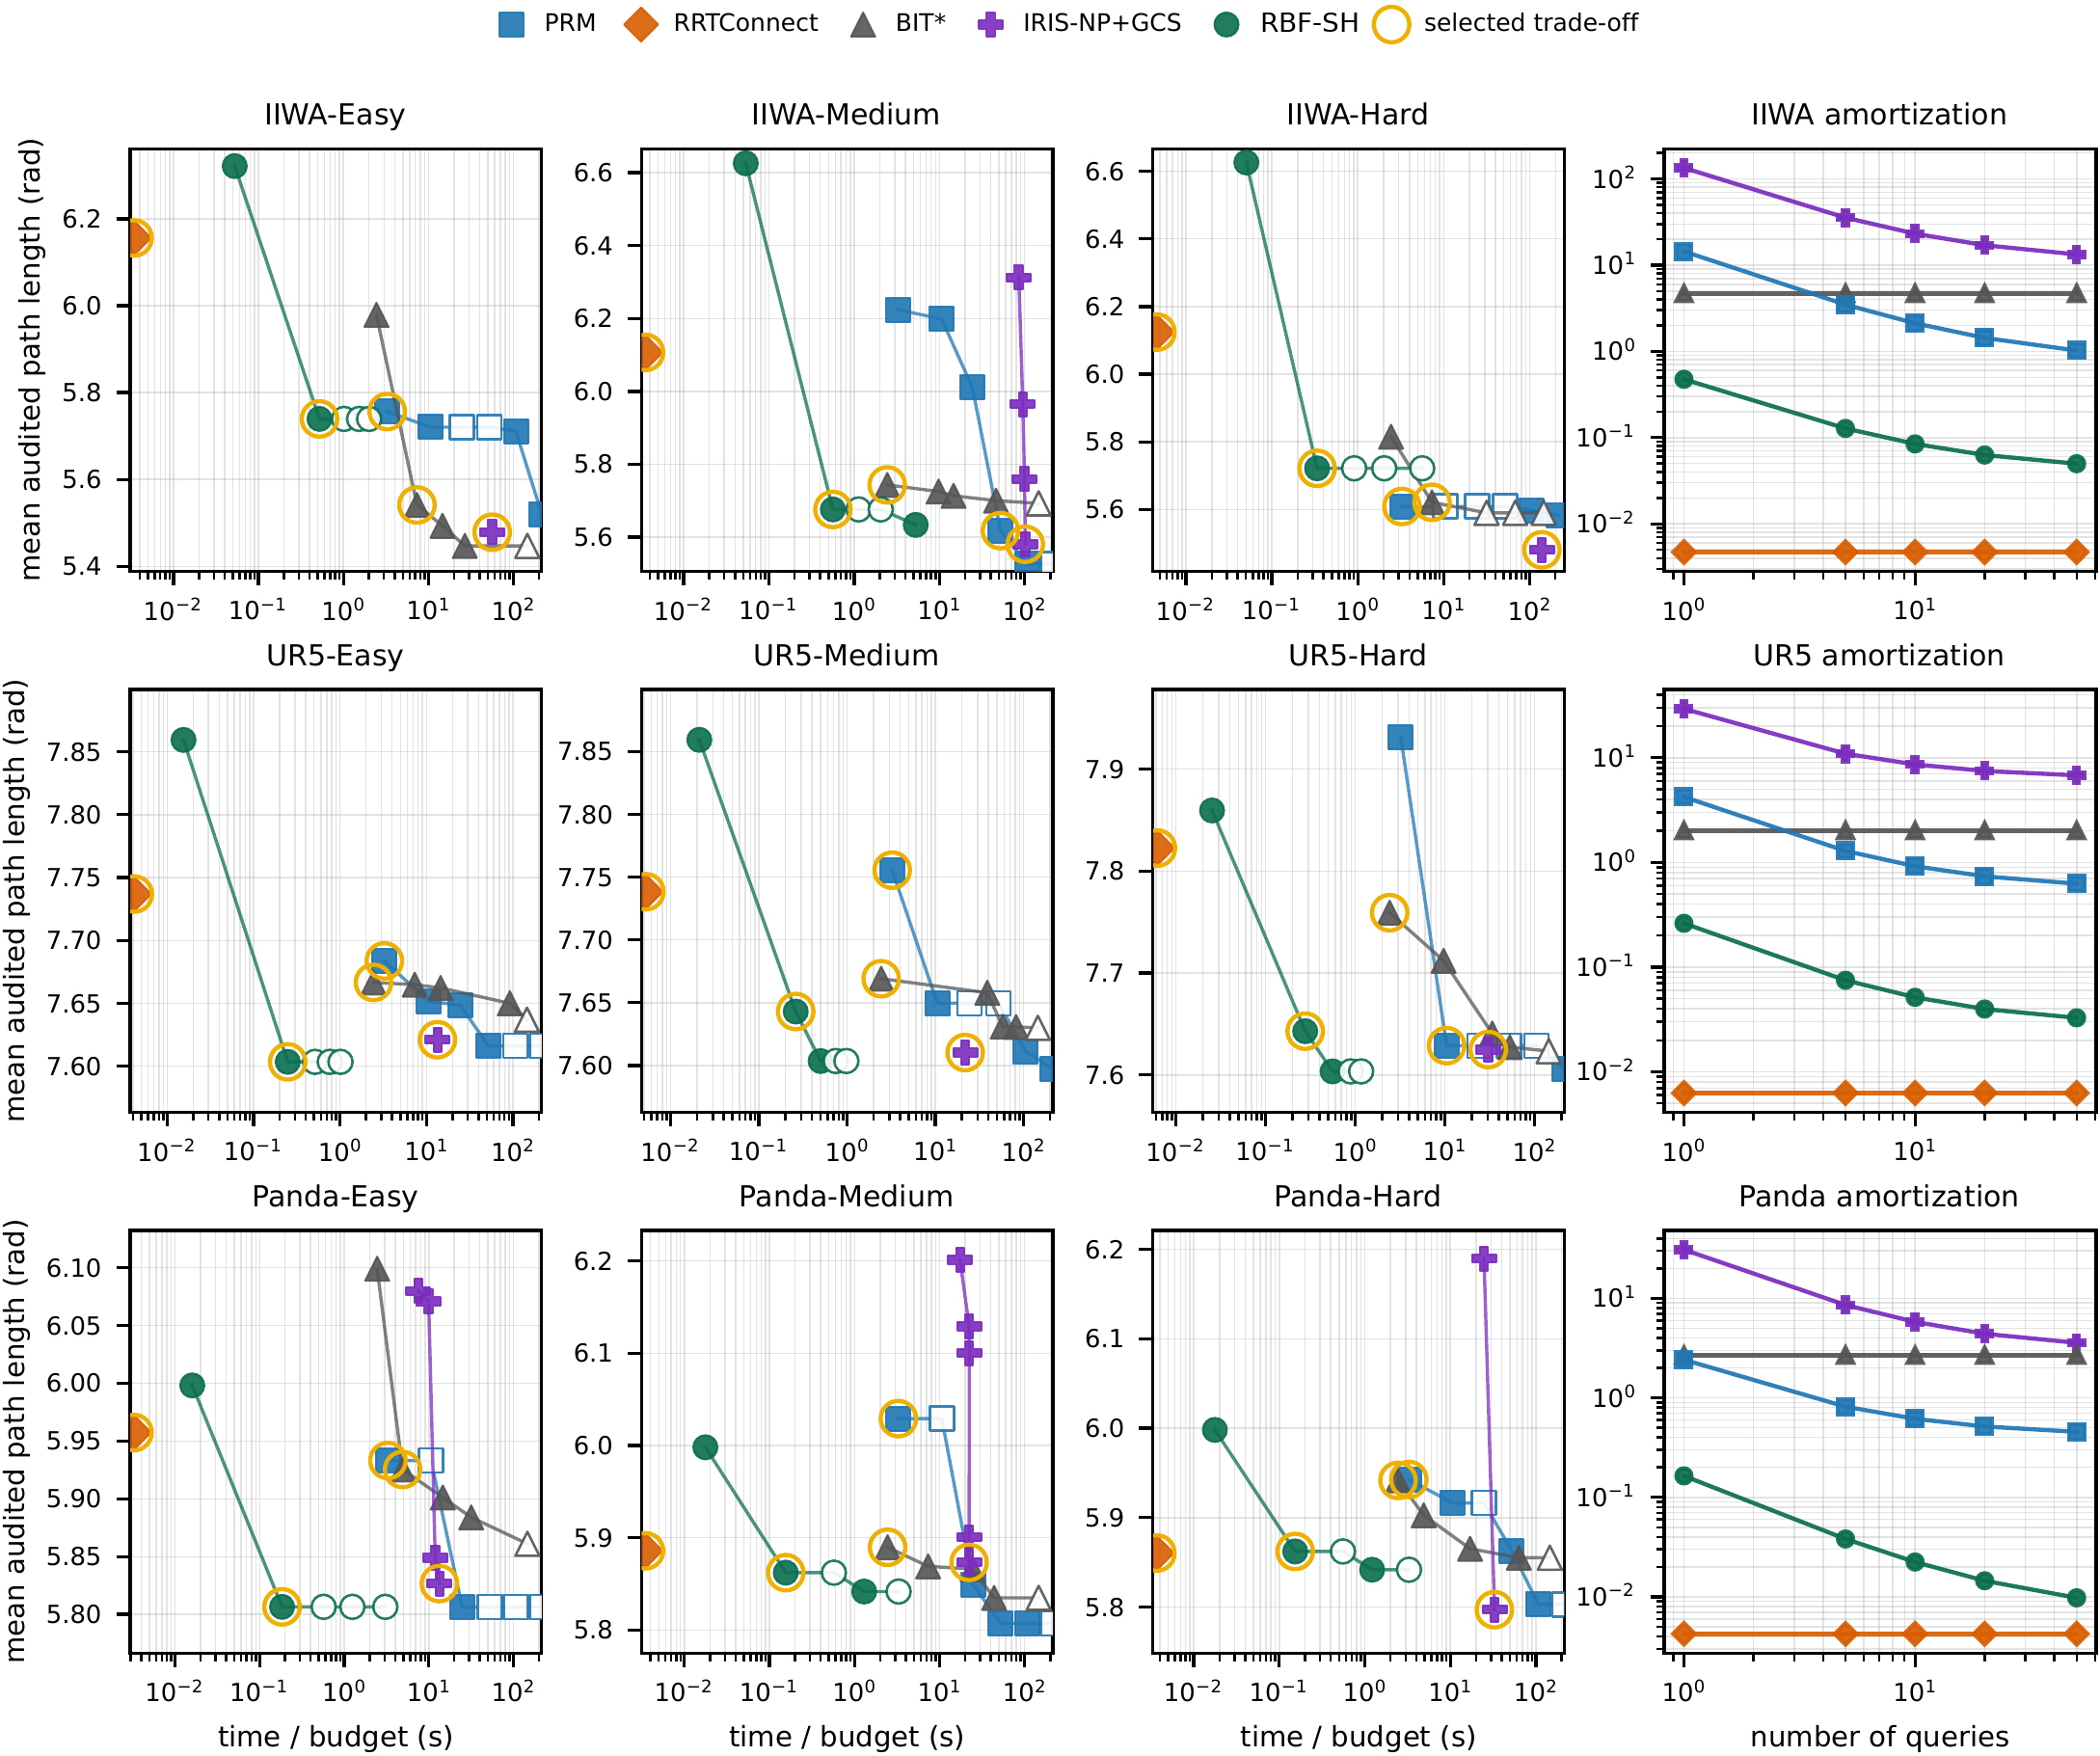
\includegraphics[width=0.89\textwidth]{generated/fig_tro_random_anytime_tradeoff_clean.png}%
  }{%
    \fbox{\parbox{0.92\textwidth}{\centering
    \vspace{0.7em}
    Missing the random-scene anytime-tradeoff figure asset.\\
    Regenerate the figure before compiling the manuscript.
    \vspace{0.7em}}}%
  }
  \caption{Balanced random-scene final-audited design-point trade-off on IIWA, UR5, and Panda. In the trade-off panels, points nearer the lower-left corner combine lower charged time with shorter audited path length. Filled markers indicate incumbent-improving checkpoints; open markers show a sparse representative subset of nonimproving checkpoints. Gold rings mark the rows reported in \cref{tab:tro_main_random_best_tradeoff}. Small offsets separate nearly coincident IRIS-NP+GCS and PRM points.}
  \label{fig:tro_random_anytime_tradeoff}
  \vspace{1em}
  % Auto-generated from current anytime trade-off artifacts.
\begin{minipage}{\textwidth}
\centering
\refstepcounter{table}
\makeatletter\def\@currentlabelname{Common-rule tabulated random-scene rows}\makeatother
\addcontentsline{lot}{table}{\protect\numberline{\Roman{table}}Common-rule tabulated random-scene rows from Fig.~\ref{fig:tro_random_anytime_tradeoff}.}
\label{tab:tro_main_random_best_tradeoff}
{\small\textsc{Table~\Roman{table}}\par}
{\small Common-rule tabulated random-scene rows from Fig.~\ref{fig:tro_random_anytime_tradeoff}. Gold rings identify these rows only to expose detailed numeric values; the full curves remain the primary evidence. Each method and scenario is evaluated on its full curve, and the table lists one readable slice because the complete checkpoint data are too extensive to print in full. Among points within 8\% of the shortest audited path, the rule minimizes a single path/log-time utility. BIT* rows are taken from the audited monotone incumbent checkpoint trace under the same 0.01 OMPL planning/simplify and fixed-resolution final-audit segment step.\par}
\vspace{0.2em}
\footnotesize
\setlength{\tabcolsep}{0.72pt}
\renewcommand{\arraystretch}{0.96}
\begin{tabular}{@{}lrrr|rrr|rrr|rr|rr@{}}
\toprule
  & \multicolumn{3}{c}{\textbf{\footnotesize \shortstack{SBF-SH}}} & \multicolumn{3}{c}{\textbf{\footnotesize \shortstack{IRIS-NP+GCS}}} & \multicolumn{3}{c}{\textbf{\footnotesize \shortstack{PRM}}} & \multicolumn{2}{c}{\textbf{\footnotesize \shortstack{RRTConnect}}} & \multicolumn{2}{c}{\textbf{\footnotesize \shortstack{BIT*}}} \\
\cmidrule(lr){2-4}\cmidrule(lr){5-7}\cmidrule(lr){8-10}\cmidrule(lr){11-12}\cmidrule(lr){13-14}
Scenario & Build (s) & Query (s) & Path & Build (s) & Query (s) & Path & Build (s) & Query (s) & Path & Query (s) & Path & Query (s) & Path \\
\midrule
IIWA-Easy & 0.493 & 0.029 & 5.74 & 66.0 & 10.4 & 5.46 & 2.00 & 0.412 & 5.77 & 0.0042 & 6.17 & 6.03 & 5.52 \\
IIWA-Medium & 0.509 & 0.054 & 5.68 & 126 & 11.7 & 5.56 & 37.0 & 1.42 & 5.64 & 0.0043 & 6.13 & 2.01 & 5.72 \\
IIWA-Hard & 0.297 & 0.040 & 5.72 & 177 & 10.5 & 5.46 & 2.00 & 0.415 & 5.63 & 0.0056 & 6.14 & 6.03 & 5.60 \\
UR5-Easy & 0.222 & 0.026 & 7.60 & 12.1 & 6.04 & 7.62 & 2.00 & 0.413 & 7.69 & 0.0050 & 7.74 & 2.01 & 7.66 \\
UR5-Medium & 0.233 & 0.028 & 7.64 & 23.5 & 5.66 & 7.60 & 2.00 & 0.413 & 7.76 & 0.0063 & 7.74 & 2.01 & 7.66 \\
UR5-Hard & 0.246 & 0.031 & 7.64 & 33.4 & 7.27 & 7.62 & 7.00 & 0.832 & 7.64 & 0.0075 & 7.83 & 2.01 & 7.75 \\
Panda-Easy & 0.178 & 0.0061 & 5.81 & 15.1 & 3.03 & 5.82 & 2.00 & 0.414 & 5.94 & 0.0040 & 5.96 & 4.02 & 5.92 \\
Panda-Medium & 0.148 & 0.0074 & 5.86 & 27.1 & 3.02 & 5.87 & 2.00 & 0.416 & 6.04 & 0.0042 & 5.89 & 2.01 & 5.88 \\
Panda-Hard & 0.147 & 0.0064 & 5.86 & 41.3 & 3.00 & 5.79 & 2.00 & 0.416 & 5.95 & 0.0045 & 5.87 & 2.01 & 5.93 \\
\bottomrule
\end{tabular}
\end{minipage}

\end{figure*}

\Cref{fig:tro_random_anytime_tradeoff} reports balanced easy/medium/hard IIWA, UR5, and Panda scenes on the same platform as Shelf+IIWA. The random-scene comparison again uses the common final-path post-processing and fixed 0.01 joint-space audit protocol; OMPL planners use the same segment step for planning and final simplify. RRTConnect is one maximum-timeout call per scene/trial with no restart accounting, while BIT* is one fixed-timeout call with incumbent checkpoints summarized as a monotone anytime curve. For \cref{tab:tro_main_random_best_tradeoff}, each method and scenario contributes one row chosen by a common rule: among points within 8\% of the shortest audited path, select the minimum of a single path/log-time utility.

The easy/medium/hard labels control obstacle count and nominal clutter, not a guaranteed runtime ordering. In easy scenes the larger free space can leave sampling-based planners and region builders with more irrelevant volume to explore before the useful corridor is resolved. As a result, an easy panel can charge more build or search time than the corresponding medium or hard panel even under the same planner settings.

Under this shared tabulation rule, \cref{tab:tro_main_random_best_tradeoff}
summarizes the reported trade-offs. In this pipeline-level comparison, the
\rbf{} rows build in 0.147--0.509~s and query in 0.0061--0.054~s; the
corresponding PRM rows require 2.00--37.0~s charged build, and the
corresponding IRIS-NP+GCS rows require 12.1--177~s. The price is a path-quality
gap that varies by robot and scene: at the tabulated rows, RBF-SH remains within
0.092~rad of PRM and within 0.217~rad of BIT*, but IRIS-NP+GCS and BIT* give
shorter audited paths in several panels. This is the central empirical message:
\rbf{} trades very low reusable build/query cost for near-baseline, not
uniformly best, audited path length. Because the IRIS seed generation differs between
Shelf+IIWA and the random scenes, these timings quantify the current end-to-end
pipelines rather than seed-independent convex-region construction cost.

Against the stronger single-query reference BIT*, \rbf{} occupies a different point in the design space: reusable build with near-baseline path quality at much smaller online planning budgets. RRTConnect serves as a no-build latency floor, either connecting within the maximum timeout or contributing a failed trial. BIT* provides the single-query quality curve through the audited monotone incumbent extracted from one long run, with the hollow markers in the figure showing a sparse representative subset of nonimproving checkpoints. This comparison shows the observed path-length/time trade-off of the implemented \rbf{} pipeline, while leaving a broader strategy-ablation study for future work.

Accounting matches the deployment regimes: \rbf{} contributes reusable link-envelope box-forest build, PRM reusable roadmap build, IRIS-NP+GCS convex-region build before GCS query, and RRTConnect/BIT* no reusable build phase. The remaining \rbf{} gaps to the shortest single-query points mainly reflect the absence of a dedicated post-corridor path optimizer.

\subsection{Mechanism Studies: Envelopes and Cache}\label{sec:exp_mechanisms}

\begin{figure*}[t]
  \centering
  \begin{minipage}[t]{0.48\textwidth}
    \vspace{0pt}
    \centering
    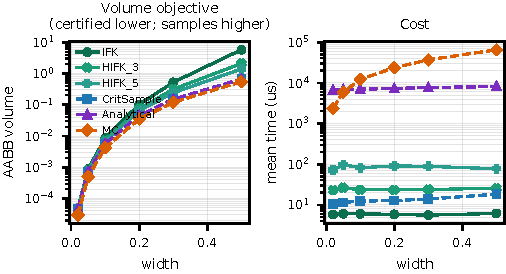
\includegraphics[width=0.96\linewidth]{generated/fig_tro_evidence_validation_tradeoff.pdf}
    \captionof{figure}{Endpoint interval-envelope source study for link-envelope box validation. Left: endpoint AABB volume versus fixed width. Right: mean evaluation time versus fixed width.}
    \label{fig:tro_evidence_validation_tradeoff}
    \vspace{1em}
    % Auto-generated from the endpoint interval-envelope artifact.
\begingroup
\centering
\captionof{table}{Endpoint-interval AABB source comparison at fixed widths.}
\label{tab:tro_main_evidence_validation}
\scriptsize
\setlength{\tabcolsep}{2.0pt}
\renewcommand{\arraystretch}{0.76}
\begin{tabular}{@{}llrrr@{}}
\toprule
Width & Source & $V$ (m$^3$) & Mean ($\mu$s) & Max gap (m) \\
\midrule
0.02 & IFK & 0.000050 & 5.7 & 0.0000 \\
0.02 & HIFK\_3 & 0.000047 & 23.0 & 0.0000 \\
0.02 & HIFK\_5 & 0.000047 & 71.7 & 0.0000 \\
0.02 & CritSample & 0.000046 & 10.4 & 0.0000 \\
0.02 & Analytical & 0.000046 & 6744.8 & 0.0000 \\
0.02 & MC & 0.000029 & 2348.3 & 0.0061 \\
\addlinespace
0.05 & IFK & 0.000873 & 6.0 & 0.0000 \\
0.05 & HIFK\_3 & 0.000801 & 26.3 & 0.0000 \\
0.05 & HIFK\_5 & 0.000765 & 96.4 & 0.0000 \\
0.05 & CritSample & 0.000713 & 11.5 & 0.0002 \\
0.05 & Analytical & 0.000714 & 6855.4 & 0.0000 \\
0.05 & MC & 0.000500 & 5850.2 & 0.0129 \\
\addlinespace
0.10 & IFK & 0.0085 & 6.0 & 0.0000 \\
0.10 & HIFK\_3 & 0.0071 & 23.4 & 0.0000 \\
0.10 & HIFK\_5 & 0.0067 & 81.8 & 0.0000 \\
0.10 & CritSample & 0.0057 & 12.3 & 0.0012 \\
0.10 & Analytical & 0.0057 & 6999.9 & 0.0000 \\
0.10 & MC & 0.0042 & 12197.6 & 0.0277 \\
\addlinespace
0.20 & IFK & 0.1025 & 5.8 & 0.0000 \\
0.20 & HIFK\_3 & 0.0754 & 23.4 & 0.0000 \\
0.20 & HIFK\_5 & 0.0649 & 90.5 & 0.0000 \\
0.20 & CritSample & 0.0451 & 12.8 & 0.0052 \\
0.20 & Analytical & 0.0453 & 7249.9 & 0.0000 \\
0.20 & MC & 0.0351 & 23648.7 & 0.0702 \\
\addlinespace
0.30 & IFK & 0.5235 & 5.6 & 0.0000 \\
0.30 & HIFK\_3 & 0.3164 & 23.7 & 0.0000 \\
0.30 & HIFK\_5 & 0.2419 & 88.5 & 0.0000 \\
0.30 & CritSample & 0.1497 & 13.8 & 0.0126 \\
0.30 & Analytical & 0.1506 & 7688.6 & 0.0000 \\
0.30 & MC & 0.1204 & 36783.7 & 0.0869 \\
\addlinespace
0.50 & IFK & 5.769 & 6.1 & 0.0000 \\
0.50 & HIFK\_3 & 2.091 & 25.8 & 0.0000 \\
0.50 & HIFK\_5 & 1.401 & 77.1 & 0.0000 \\
0.50 & CritSample & 0.6564 & 18.3 & 0.0324 \\
0.50 & Analytical & 0.6665 & 8107.6 & 0.0030 \\
0.50 & MC & 0.5485 & 65157.7 & 0.1122 \\
\bottomrule
\end{tabular}
\par
\endgroup

  \end{minipage}\hfill
  \begin{minipage}[t]{0.48\textwidth}
    \vspace{0pt}
    \centering
    % Auto-generated from the width-wise CritSample link-envelope representation artifact.
\begingroup
\centering
\captionof{table}{Width-wise CritSample link-envelope comparison under the same $S=4$ short-link split.}
\label{tab:tro_link_envelopes}
\label{tab:tro_link_envelope_widthwise}
\scriptsize
\setlength{\tabcolsep}{2.2pt}
\renewcommand{\arraystretch}{0.82}
\begin{tabular}{@{}llrrr@{}}
\toprule
Width & Envelope & $V$ (m$^3$) & Eval ($\mu$s) & Collision ($\mu$s) \\
\midrule
0.02 & LinkIAABB & 0.0017 & 0.5 & 0.2 \\
0.02 & KDOP26 & 0.000706 & 1.3 & 0.3 \\
0.02 & SupportHull & 0.000424 & 0.5 & 0.4 \\
\addlinespace
0.05 & LinkIAABB & 0.0056 & 0.5 & 0.2 \\
0.05 & KDOP26 & 0.0041 & 1.3 & 0.4 \\
0.05 & SupportHull & 0.0035 & 0.5 & 0.5 \\
\addlinespace
0.10 & LinkIAABB & 0.0229 & 0.5 & 0.2 \\
0.10 & KDOP26 & 0.0205 & 1.3 & 0.4 \\
0.10 & SupportHull & 0.0192 & 0.5 & 0.9 \\
\addlinespace
0.20 & LinkIAABB & 0.1255 & 0.5 & 0.2 \\
0.20 & KDOP26 & 0.1214 & 1.3 & 0.5 \\
0.20 & SupportHull & 0.1189 & 0.4 & 0.9 \\
\addlinespace
0.30 & LinkIAABB & 0.3678 & 0.5 & 0.3 \\
0.30 & KDOP26 & 0.3621 & 1.3 & 0.6 \\
0.30 & SupportHull & 0.3586 & 0.4 & 1.3 \\
\addlinespace
0.50 & LinkIAABB & 1.465 & 0.6 & 0.4 \\
0.50 & KDOP26 & 1.457 & 1.5 & 0.9 \\
0.50 & SupportHull & 1.452 & 0.4 & 2.4 \\
\bottomrule
\end{tabular}
\par
\endgroup

    \vspace{1em}
    % Auto-generated from the IIWA incremental LECT reuse artifact.
\begingroup
\centering
\captionof{table}{Random IIWA LECT reuse under the paper-facing CritSample endpoint source and an approximately 250-box target regime. Warm rows use blind random-obstacle prewarm scenes; Cold and Warm replay the same validation/split route. LECT hit reports external prewarm materialization hits for Warm and cached-envelope hits for Replay. Speedup charges only the target build.}
\label{tab:tro_main_lect_reuse}
\scriptsize
\setlength{\tabcolsep}{1.4pt}
\renewcommand{\arraystretch}{0.82}
\begin{tabular}{@{}lrrrr@{}}
\toprule
Regime & Off./pop. (s) & LECT hit (\%) & Build (s) & Speedup \\
\midrule
Cold & -- & 0.0 & 0.249 & 1.00$\times$ \\
Warm & 0.394 & 23.0 & 0.232 & 1.07$\times$ \\
Warm & 0.758 & 24.7 & 0.235 & 1.06$\times$ \\
Warm & 1.793 & 26.9 & 0.225 & 1.11$\times$ \\
Warm & 3.468 & 28.5 & 0.228 & 1.09$\times$ \\
Warm & 19.980 & 33.8 & 0.219 & 1.14$\times$ \\
Replay & 0.322 & 96.9 & 0.111 & 2.23$\times$ \\
\bottomrule
\end{tabular}
\par
\endgroup

  \end{minipage}
\end{figure*}

\paragraph{Endpoint sources.}
\Cref{tab:tro_main_evidence_validation} summarizes the endpoint
interval-envelope source comparison used to choose the geometric inputs for
RBF-SH. The table reports endpoint-interval AABB volume, mean evaluation time,
and maximum gap to the sampled reference union at each fixed width used in the
standalone endpoint study. \Cref{fig:tro_evidence_validation_tradeoff}
visualizes the same width-wise trade-off. In this updated table, the certified
outer-bound baselines are IFK and two representative hierarchical
variants, HIFK\_3 and HIFK\_5, so smaller volume is better for those rows; CritSample,
Analytical, and MC estimate the sampled reference union, so larger volume is
better there. All three certified AA sources remain gap-free against the
sampled reference union over the reported widths. HIFK\_3 already removes
most of IFK's wide-box slack at modest extra cost, and HIFK\_5 pushes
that trade-off further: at width 0.50~rad the mean endpoint volume drops from
5.769~m$^3$ for IFK to 2.091~m$^3$ for HIFK\_3 and 1.401~m$^3$ for
HIFK\_5, while mean endpoint cost rises from 6.1 to 25.8 to
77.1~$\mu$s. CritSample still tracks Analytical much more closely than any of
the certified AA sources on wide boxes, reaching 0.6564 versus 0.6665~m$^3$
at 0.50~rad while remaining orders of magnitude cheaper (18.3 versus
8107.6~$\mu$s), but it remains an advisory rather than certified bound.

\paragraph{Link-envelope representations.}
The envelope microkernel fixes the endpoint source to CritSample and asks how
the same endpoint boxes should be lifted to link-sweep envelopes.
\Cref{tab:tro_link_envelope_widthwise} compares LinkIAABB, KDOP26, and pure
SupportHull at the common short-link split $S=4$. The table reports uninflated
short-link record volume, envelope construction time, and envelope-only
obstacle-check time. The representation trade-off motivates the loose-to-tight
RBF-SH cascade used in the planning experiments: cheap AABB rejection handles
most pairs first, KDOP26 slabs provide a mid-phase for survivors, and
SupportHull/GJK is reserved for the small set that still needs the tightest
geometric witness.

\paragraph{LECT reuse.}
\Cref{tab:tro_main_lect_reuse} reports LECT as a runtime optimization rather
than as the main experimental claim. Warm rows prewarm LECT on blind
random-obstacle scenes and then run a fresh route-matched target build on the
held-out target scene. As the random-scene prewarm budget grows, the LECT hit
rate rises from 23.0\% to 33.8\% and the target-build median falls from
0.249~s to 0.219~s, a modest but measurable gain. Replay is the same-scene
upper reference: it yields 96.9\% cached-envelope hit and 2.23$\times$
whole-build speedup. These numbers support LECT as a selective cache for
revisited expensive envelope records, while the main planning conclusions come
from the anytime trade-off figures above.

\paragraph{RBF-only no-grid diagnostics.}
To isolate the lifelong-cache protocol from the broader planning pipeline, the
appendix also reports a dedicated RBF-only diagnostic suite after the no-grid
cleanup. \Cref{tab:tro_appendix_rbf_only_cache_mechanism} shows that the d18
prewarm now charges FK/link-envelope materialization only on the leaf layer:
the first pass stores \TroRbfOnlyEFiveEvidence{} evidence records while directly
materializing \TroRbfOnlyEFiveLeafFk{} leaf records, and the reopen pass reuses
\TroRbfOnlyEFiveReopenReuse{} cached leaf records without fresh FK work above
the leaves. On the Shelf+IIWA appendix sweep, all
\TroRbfOnlySweepFullPassRows{} rows pass strict audit; the best row is
\TroRbfOnlySweepBestEnvelope{} at budget \TroRbfOnlySweepBestBudget{}, with
\TroRbfOnlySweepBestBuild~s build, \TroRbfOnlySweepBestQueryMs~ms query, and
\TroRbfOnlySweepBestReuse{} cached-evidence hits
(\cref{tab:tro_appendix_rbf_only_sweep}). Under the reviewer-safe warm-cache
protocol, the Shelf+IIWA warm row builds in \TroRbfOnlyShelfWarmBuild~s with
\TroRbfOnlyShelfWarmExternalReuse{} external evidence hits and
\TroRbfOnlyShelfWarmQueryMs~ms median query time, while the balanced
random-scene warm rows span \TroRbfOnlyEFourWarmBuildMin--\TroRbfOnlyEFourWarmBuildMax~s
build and \TroRbfOnlyEFourWarmQueryMinMs--\TroRbfOnlyEFourWarmQueryMaxMs~ms
query with at least \TroRbfOnlyEFourWarmAuditMin\% audit success
(\cref{tab:tro_appendix_rbf_only_warm_reuse}). Rechecking the earlier UR5
audit failures showed that they came from an under-budgeted random-scene RBF
runner rather than from center-to-center stitching or shortcut drift;
restoring the original random-scene growth and parallelism budget removed that
failure mode. The remaining IIWA warm rows are therefore best read as
final-audited diagnostics rather than as reusable-corridor builds, since some
scenes still succeed only through the bounded repair stage after an empty
forest build.


\subsection{Dynamic-Update Capability Study}\label{sec:exp_dynamic_updates}

\Cref{tab:tro_dynamic_rebuild} summarizes the local update procedure on the
same balanced random-scene construction used in the anytime study. This
creates two matched edit paths: insertion from easy to medium to hard, and
deletion from hard to medium to easy. The warm baseline is measured per
transition, not as a cumulative path artifact: the source scene first populates
an isolated fingerprint-cache namespace, and the reported warm time is then a
fresh target-scene \texttt{build\_coverage} call from that cache. This matches
the random-scene warm-cache accounting and avoids carrying hidden in-memory
state from earlier transitions.

\begin{table*}[t]
\centering
\caption{Leaf-sweep--RRT dynamic updates on constrained random AABB scenes sampled inside the Exp.~4 d23 canonical inverse-root domain. Update time excludes final query audit; warm is a fresh target-scene leaf-refine rebuild from the same read-only d23 evidence cache.}
\label{tab:tro_dynamic_rebuild}
\footnotesize
\setlength{\tabcolsep}{3.0pt}
\renewcommand{\arraystretch}{0.98}
\resizebox{\textwidth}{!}{%
\begin{tabular}{@{}llrrrrrrrrrrrr@{}}
\toprule
Transition & Edit & Update (ms) & Warm (ms) & Speedup & Invalid & Promoted & Cache cand. & Cache rej. & Repair boxes & Fallback & Islands & Seg. & Ok \\
\midrule
easy->medium & insert & 20.7 & 403.8 & 19.24 & 208 & 0 & 0 & 0 & 0 & 4/8 & 1 & 0.00 & 8/8 \\
medium->hard & insert & 20.8 & 432.0 & 17.25 & 313 & 0 & 0 & 0 & 0 & 4/8 & 1 & 0.00 & 8/8 \\
hard->medium & delete & 4.3 & 394.7 & 82.50 & 0 & 0 & 8054 & 0 & 0 & 0/8 & 1 & 0.00 & 8/8 \\
medium->easy & delete & 3.5 & 362.5 & 98.81 & 0 & 0 & 7108 & 0 & 0 & 0/8 & 1 & 0.00 & 8/8 \\
\bottomrule
\end{tabular}
}
\end{table*}


The incremental update is consistently faster than this cache-warm rebuild
baseline on the five-seed IIWA dynamic protocol. Insertion medians are
9.5~ms for easy$\rightarrow$medium and 36.4~ms for
medium$\rightarrow$hard, compared with 90.2~ms and 70.2~ms for warm rebuilds.
Deletion is cheaper still because previously accepted boxes remain valid when
obstacles are removed: hard$\rightarrow$medium takes 1.4~ms and
medium$\rightarrow$easy takes 0.33~ms, versus 58.1~ms and 46.4~ms warm
target rebuilds. The apparent build-time ordering is driven by transition
geometry and scene topology: the target
easy warm rebuild is the shortest target rebuild after cache isolation, while
easy$\rightarrow$medium is longer because it measures rebuilding the medium
target from the easy source scene. Incremental audit succeeds on all insertion
and medium$\rightarrow$easy deletion cases and on 4/5 hard$\rightarrow$medium
deletions; failed audits remain failures under the same accounting used
elsewhere in the paper.

\section{Conclusion}\label{sec:conclusion}

This paper presented \rbf{}, a link-envelope-guided box-forest method for fast
multi-query manipulator planning. Its geometric core maps endpoint interval
envelopes to link interval envelopes via capsule Minkowski decomposition and
convex-hull generator bounding; an RRT-inspired grower builds a scene-specific
box forest into a corridor graph queried by graph search and local refinement;
LECT optionally caches kinematic envelope records to reduce repeated
materialization cost. On the studied Shelf+IIWA and balanced IIWA/UR5/Panda
workloads, the implemented \rbf{} pipeline offers a low reusable build/query
design point---below 1.1~s build and 0.11~s query---with near-baseline audited
path lengths under common post-processing and fixed-resolution final audit.

\paragraph{Limitations.}
The box-corridor guarantee (\cref{thm:corridor_certificate}) is conditional on
conservative IFK validation and path containment inside the validated box union;
the main reported rows do not claim that condition, and no
corridor-containment fields were stored in the current artifacts. The
paper-wide 663/668 audit count reflects fixed-resolution (0.01 joint-space
step) empirical checks, not continuous safety guarantees. \rbf{} is best
viewed as an integration of link-envelope filtering, adaptive cell
decomposition, and frontier-biased sampling; the main anytime curves are
full-pipeline results that do not isolate the envelope primitive, box
representation, or grower heuristics. Cross-scene LECT gains are modest at the
tested prewarm budgets; the dynamic-update result is a capability study on the
reported IIWA edit protocol, not a broad claim about dynamic scenes across
robots or edit distributions.

\paragraph{Scope and Future Work.}
The empirical scope covers one shelf workload, balanced IIWA/UR5/Panda random
scenes at 50 seeds per robot/difficulty setting, and the present budget grid;
distributional generalization, grower ablations, worker-count sensitivity, and
narrow-clearance stress tests remain uncharacterized. Important extensions
include broader scene families and larger seed sets, explicit box-containment
coverage instrumentation, broader audit-step robustness checks,
containment-preserving path optimization, stronger forest connectivity, and
richer cache-transfer and dynamic-update benchmarks.

\appendices

\section{RBF-only No-grid Diagnostics}\label{app:rbf_only_nogrid}

These appendix tables record the reviewer-safe RBF-only protocol used in the
final reruns: d18 prewarm materializes FK/link-envelope evidence only on the
leaf layer, Shelf+IIWA warm rows keep the prewarmed cache read-only, and
balanced random-scene rows may backfill newly materialized online evidence into
the active database.

\IfFileExists{generated/tab_tro_rbf_only_cache_mechanism.tex}{\begin{table}[t]
\centering
\caption{RBF-only Gate 0 and lifelong-cache mechanism status after the no-grid refactor. In E5, FK/link-envelope materialization is charged only on the target leaf layer; parent layers are reconstructed by child-hull propagation during checkpoint.}
\label{tab:tro_appendix_rbf_only_cache_mechanism}
\footnotesize
\setlength{\tabcolsep}{2.40pt}
\renewcommand{\arraystretch}{0.95}
\begin{tabular}{llrrrrrrr}
\toprule
Stage & Status & Depth & Leaf FK & Nodes & Evidence & Wall s & Reuse & Cache GiB \\
\midrule
E5 prewarm & pass & 18 & 262144 & 524287 & 524287 & 33.82 & 0 & 0.3113 \\
E5 reopen & pass & 18 & 0 & 524287 & 524287 & 1.794 & 262144 & 0.3113 \\
\bottomrule
\end{tabular}
\end{table}
}{}

\IfFileExists{generated/tab_tro_rbf_only_sweep.tex}{\begin{table}[t]
\centering
\caption{Standalone link-envelope representation summary over the 2400-box fixed-width corpus. The table reports per-box staged materialization cost for LinkIAABB, KDOP26, SupportHull, and the AABB-first chain variants; the escalation column is the fraction of boxes that must run at least one post-AABB stage.}
\label{tab:tro_appendix_rbf_only_sweep}
\footnotesize
\setlength{\tabcolsep}{2.30pt}
\renewcommand{\arraystretch}{0.95}
\begin{tabular}{rllrr}
\toprule
Rank & Representation & Payload & Build/box us & Escalation \% \\
\midrule
1 & LinkIAABB & 384.0 B & 0.6809 & -- \\
2 & KDOP26 & 1.62 KB & 1.942 & -- \\
3 & SupportHull & 832.0 B & 1.767 & -- \\
4 & AABB->KDOP26 & 854.8 B & 1.273 & 28.3 \\
5 & AABB->SupportHull & 619.4 B & 1.254 & 28.3 \\
6 & AABB->KDOP26->SupportHull & 1.06 KB & 1.847 & 28.3 \\
\bottomrule
\end{tabular}
\end{table}
}{}

\IfFileExists{generated/tab_tro_rbf_only_warm_reuse.tex}{\begin{table*}[t]
\centering
\caption{RBF-only warm-versus-cold baselines under the reviewer-safe lifelong-cache protocol. Shelf rows read only the prewarmed external d18 snapshot-backed evidence source and disable active-database backfill; random-scene rows may persist newly materialized online evidence to the active database.}
\label{tab:tro_appendix_rbf_only_warm_reuse}
\small
\setlength{\tabcolsep}{2.00pt}
\resizebox{\textwidth}{!}{%
\begin{tabular}{llllrrrrrrrr}
\toprule
Exp. & Scene & Mode & Backfill & Wall s & Plan s & Maint s & Query ms & Audit & Repairs & Ext reuse & Active reuse \\
\midrule
E2 & Shelf+IIWA & Cold & no & 1.820 & 1.799 & 0.0213 & 15.98 & 1/1 & 1 & 0 & 4954 \\
E2 & Shelf+IIWA & Warm d18 & no & 1.812 & 1.791 & 0.0212 & 15.57 & 1/1 & 1 & 3420 & 1809 \\
E2 & Random IIWA (easy) & Cold & yes & 0.1821 & 0.1562 & 0.0259 & 2.300 & 1/1 & 0 & 0 & 3249 \\
E2 & Random IIWA (easy) & Warm d18 & yes & 0.1727 & 0.1467 & 0.0259 & 2.332 & 1/1 & 0 & 3002 & 664 \\
E3 & Shelf+IIWA & Cold & no & 1.587 & 1.553 & 0.0333 & 3.679 & 5/5 & 0 & 0 & 10688 \\
E3 & Shelf+IIWA & Warm d18 & no & 1.588 & 1.555 & 0.0335 & 3.568 & 5/5 & 0 & 7201 & 3946 \\
\bottomrule
\end{tabular}
}
\end{table*}
}{}

\bibliographystyle{IEEEtran}
\bibliography{references}

\end{document}